\documentclass[11pt]{article}

\usepackage{geometry}
\usepackage[T1]{fontenc}
\usepackage[utf8]{inputenc}
\usepackage{lmodern}
\usepackage{amsmath,amssymb,amsthm,amsfonts}
\usepackage{booktabs}
\usepackage{graphicx}
\usepackage{siunitx}
\usepackage[numbers]{natbib}
\usepackage{hyperref}
\usepackage[nameinlink,noabbrev]{cleveref}
\usepackage{setspace}
\usepackage{subcaption}
\usepackage{placeins}
\geometry{a4paper,margin=2.5cm}
\usepackage{changepage}
\usepackage[normalem]{ulem}
\usepackage{authblk}
\usepackage{array}
\usepackage[table]{xcolor}
% Revisions that unpack dense attributive modifiers are highlighted in blue.
\newenvironment{review}{\begingroup\color{blue}}{\endgroup}
\usepackage{tabularx}
\usepackage{tikz}
\usetikzlibrary{arrows.meta,positioning,plotmarks}
\InputIfFileExists{generated/spoofing_empirical_macros.tex}{}{}

\onehalfspacing
\hypersetup{
    colorlinks=true,
    linkcolor=blue,
    citecolor=blue,
    urlcolor=blue,
    pdftitle={Detecting Spoofing in Electronic Markets},
    pdfauthor={Daniele Maria Di Nosse, Francesco Gigante, Antonio Russo, Fabrizio Lillo}
}


\title{An Auditable Market-Microstructure Framework for Spoofing-Compatible Sequence Detection}
\author[1]{Daniele Maria Di Nosse\textsuperscript{\dag}}
\author[2]{Francesco Gigante}
\author[2]{Antonio Russo}
\author[1]{Fabrizio Lillo}

\affil[1]{Scuola Normale Superiore, Pisa, Italy}
\affil[2]{Consob, Rome, Italy}
\date{\today}

\begin{document}

\maketitle
\begin{center}
  \footnotesize
  \dag Corresponding author. Email: \texttt{daniele.dinosse@sns.it}
\end{center}

\begin{abstract}
How can surveillance data isolate order-book sequences that are compatible with spoofing without treating ordinary
liquidity provision as manipulation? We develop an auditable microstructure framework that reconstructs participant-attributed
order-book sequences rather than classifying isolated cancellations. It reconstructs the visible limit order book and groups
related execution messages into analytical executions, anchored either by the actor's passive resting-order execution or by the actor's
aggressive execution. For each execution, the fixed candidate set contains same-actor, opposite-side orders that are active
in the top $10$ ranks immediately before the first execution and no more than $90$ seconds old. An empirical depth kernel
weights visible liquidity by book rank. The four-condition gate requires a candidate-order cancellation canonically assigned
within $2$ seconds, attributed withdrawal larger than execution quantity, positive favorable pre-execution midprice movement,
and positive cancel-anchored midprice reversion over a $2$-second horizon. We use the original client code when available and
the firm identifier only as a labelled fallback, while preserving the identity level.

In the Risanamento, Nexi, and Ferrari samples, respectively, the reconstruction identifies
\RisanamentoMatchedClusters{}, \NexiMatchedClusters{}, and \FerrariMatchedClusters{} matched executions, of which
\RisanamentoCompatibleSequences{}, \NexiCompatibleSequences{}, and \FerrariCompatibleSequences{} satisfy the strict gate.
Both passive and aggressive execution routes contribute to these sets. An exploratory comparison with $36$ timed external
alert records yields $34$ distinct subject--instrument intervals after overlapping or endpoint-sharing records are merged.
Every interval contains a recovered execution, $30$ contain an attributed withdrawal, and four contain a strict sequence.
The four strict overlaps occur only at firm scope, where the external firm maps to multiple canonical actors. These findings
support reproducible surveillance triage, but they do not constitute a statistical test, identify manipulative intent, estimate
causal effects, measure spoofing prevalence, or validate recall against independently adjudicated manipulation labels.
Legitimate liquidity provision remains an explicit alternative explanation.
\end{abstract}

\paragraph{Keywords.}
Spoofing detection; market manipulation; limit order book; high-frequency trading; anomaly detection; market maker; market microstructure

\section{Introduction}
\label{sec:introduction}
Electronic continuous double auctions organize price discovery through a limit order book (LOB). The LOB records the
visible bid and ask orders submitted by market participants and changes whenever an order is entered, amended, executed,
or cancelled. Algorithmic and high-frequency trading have increased the speed of these updates and can improve short-term
liquidity. The same speed permits large displayed positions to be submitted and withdrawn over intervals that can be
difficult to assess as complete sequences in real time.

Spoofing exploits this sequencing problem. In a stylized account, a participant submits a large order on one side of the
LOB that is not intended to execute. The displayed quantity may change observed imbalance or microprice indicators and may
prompt other participants to revise quotes or submit aggressive orders. The participant can then execute a smaller order on
the opposite side at a more favorable price and withdraw the large displayed order. The Market Abuse Regulation (MAR)
prohibits orders and behavior that create false or misleading signals about the supply of, demand for, or price of a
financial instrument \cite{EU5962014}.

The observable actions in this mechanism are not unique to spoofing. Liquidity providers also submit, amend, and cancel
orders at high frequency, and they may have high order-to-trade ratios. They remove quotes to update prices,
control inventory, or limit adverse selection. Static size thresholds, cancellation ratios, and volumetric triggers
therefore cannot by themselves distinguish manipulative conduct from legitimate liquidity provision. Such rules can
produce false positives and cannot establish the participant's intent.

\begin{review}
A deliberately broad diagnostic makes this overlap visible. \Cref{fig:actor_cancellation_rank} ranks actors by the rate at
which they cancel liquidity on the side opposite to an execution within the next two seconds. Positive rates occur in all
three samples, but the frequency and the number of supporting executions vary substantially across actors. The
statistic is deliberately agnostic about why an order was cancelled. A high value can arise from ordinary quote and
inventory management, so it is not evidence of manipulation. The dispersion instead motivates a reconstruction that asks
which rapid cancellations also belong to the more specific sequence implied by the hypothesized mechanism.
\end{review}

\begin{figure}[htbp]
    \centering
    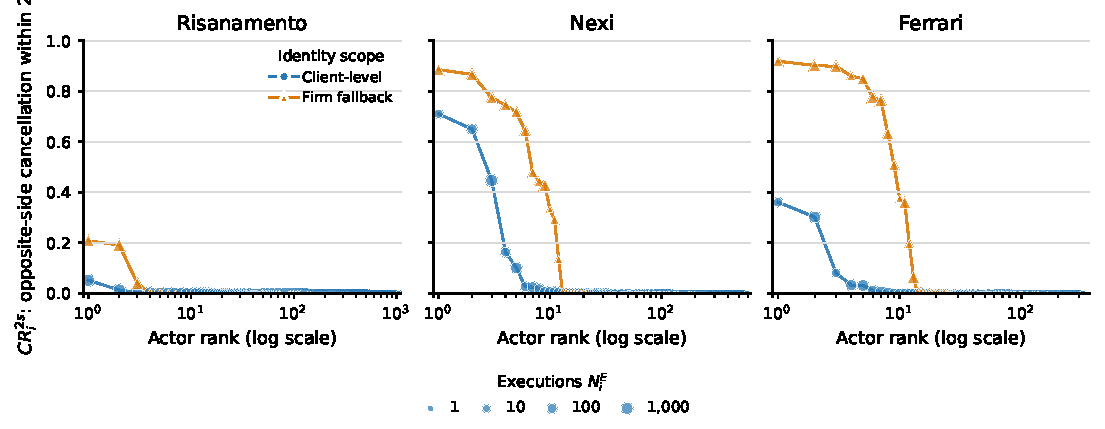
\includegraphics[width=\textwidth]{generated/actor_post_execution_cancellation_rank.pdf}
    \caption{\begin{review}Rate at which each actor cancels opposite-side liquidity within two seconds of its own execution.
    For actor $i$, the denominator $N_i^E$ contains all of its passive and aggressive executions. The numerator
    counts executions followed by at least one cancellation by the same canonical actor on the opposite side during
    $(t_c^{\mathrm{end}},t_c^{\mathrm{end}}+2\,\mathrm{s}]$. The cancellation must also follow the final constituent execution message
    in canonical source order and remain in the same trading partition. Each execution contributes at most one unit to the
    numerator, regardless of how many qualifying cancellations follow it. Each execution defines its own window, so the same
    cancellation can follow more than one nearby execution. Client-level and firm-fallback actors form two separate curves and
    are ranked from highest to lowest rate within each identity scope and instrument. The actor-rank axis is logarithmic, and
    no actor identifier is displayed. Identity follows the client-first rule: the original client code is used when
    available, with the firm identifier used only as a labelled fallback. Marker area increases with $\log(1+N_i^E)$ to
    make sample support visible; marker shape and color also distinguish the two identity scopes. No actor is removed for low
    activity. Firm fallback is a coarser scope that can pool client activity, so its rates are not directly equivalent to
    client-level rates. This broad statistic does not impose the later conditions on candidate age, the fixed candidate set,
    withdrawal size, or the price path, and it does not use WMSCI, MSCI, or the strict gate. A high rate is not evidence of
    manipulation.\end{review}}
    \label{fig:actor_cancellation_rank}
\end{figure}

This paper asks whether the observable conjunction implied by the hypothesized mechanism can be reconstructed from
participant-attributed messages without treating frequent cancellation itself as evidence of spoofing. The reconstruction
separates a broad description of displayed liquidity from the conditions used to screen events. Complete top-$10$ resting-profile
measures describe the shape of an actor's liquidity but do not determine eligibility. For each passive or aggressive execution,
we fix a candidate set of same-actor, opposite-side orders that are active in the top $10$ ranks and no more than $90$ seconds
old. An execution is matched when a cancellation of a candidate order is canonically assigned within $2$ seconds. The
four-condition gate retains only matched executions for which attributed withdrawal exceeds execution quantity, favorable
pre-execution midprice movement is positive, and cancel-anchored midprice reversion is positive over a $2$-second horizon.
Actor identity is a separate data problem: we use the original client code when present and the firm identifier only as a
fallback. Each physical cancellation is assigned to at most one execution.

\pagebreak[4]

Rapid same-actor withdrawals occur in all three samples and after both execution routes. The strict sequence is less common
because it requires the matched withdrawal to be large relative to the execution and the observed price path to satisfy both
directional conditions. This gap is the main empirical result. A mechanical withdrawal can motivate review, but it is not
equivalent to a sequence that also satisfies the size and price-path conditions of the stylized mechanism. The resulting
diagnostics support analyst triage; they are not a statistical validation, a label of manipulation, or an estimate of causal
price impact. WMSCI separately orders candidate events by the scale and speed of attributed withdrawal relative to the
execution. It does not define the four-condition gate.

The exploratory comparison with externally supplied surveillance alerts provides a separate, lower tier of evidence. The
$36$ timed source records form $34$ distinct subject--instrument intervals after overlapping or endpoint-sharing records are
merged. All $34$ intervals contain a recovered execution, $30$ contain an attributed withdrawal, and four contain a strict
sequence. The four strict overlaps occur only at firm scope, where the external firm maps to multiple canonical actors.
They therefore establish subject-scope coverage rather than exact-actor correspondence. Because the external alerts are
positive seeds rather than independently adjudicated labels, the audit measures recovery relative to the source alerts.
Exact-actor strict recall is identifiable only when external and internal identities have aligned granularity; it is not recall
against confirmed manipulation.

\section{Market Making Versus Spoofing}
\label{sec:mm_vs_spoofing}
The screening model starts from two stylized economic benchmarks. Both can generate frequent order messages and
cancellations, but they assign different roles to displayed liquidity. The contrast does not imply that every market maker
quotes symmetrically or that every spoofing episode follows one fixed pattern. It identifies observable features that can
guide surveillance.

\subsection{The Market Maker's Problem}
\label{subsec:market_maker}
A market maker supplies liquidity by posting resting orders on the bid and ask sides of the book. In a stylized
inventory-risk benchmark, the dealer earns the bid--ask spread while controlling inventory and exposure to adverse
selection. Optimal quotes therefore depend on order-arrival rates and the dealer's inventory.

Stochastic-control models often express this problem through a Hamilton--Jacobi--Bellman equation. The dealer chooses bid
and ask quotes that balance execution revenue against inventory risk. For example, a long inventory exposes the dealer to
a price decline. The dealer can respond by shifting both quotes downward: a lower ask encourages purchases from the
dealer, while a lower bid discourages further sales to the dealer. The quote adjustment depends on the midprice, the
spread required for compensation, and the penalty for inventory away from the target.

Within this benchmark, frequent cancellation is a risk-management action. The market maker cancels and reposts orders as
the midprice, adverse-selection risk, or inventory changes. The dealer generally maintains a two-sided presence near the
top of the book, although actual quoting can become asymmetric because of inventory, information, or market conditions.
Expected profits in the benchmark come primarily from spread capture rather than from deliberately inducing a directional
change in the midprice.

\subsection{The Spoofer's Problem}
\label{subsec:spoofing}
In the stylized spoofing mechanism, the participant is hypothesized to improve the price of a directional execution.
The participant displays a large order on one side of the book and submits a smaller order on the opposite side. The large
displayed order creates an asymmetric depth profile. Algorithms or traders that use bid--ask volume imbalance may interpret
this profile as short-horizon price pressure and adjust their orders. If other traders respond to the displayed asymmetry,
the resulting price movement could improve the execution of the smaller opposite-side order.

The displayed order creates a trade-off between influence and execution risk. An order near the best quote is prominent
in the book but is also more likely to execute. An order posted at Level 2, Level 3, or deeper has a buffer against
immediate execution while remaining visible in multilevel order-book data. A participant implementing the stylized
strategy may therefore distribute the large profile across deeper levels rather than place all of it at the touch.

After the smaller order executes, rapid withdrawal of the opposite-side profile is consistent with reducing subsequent
execution exposure under the hypothesized strategy. This timing distinguishes the candidate withdrawal from ordinary quote
updates: it follows the opposite-side execution rather than only changes in fair value, inventory, or adverse-selection risk.
\Cref{tab:surveillance-models} summarizes these stylized incentives; none is directly observed as intent.

\begin{table}[htbp]
\centering
\caption{Stylized differences used to construct the surveillance diagnostics. These differences describe economic
benchmarks, not observed intent or necessary conditions for either activity.}
\label{tab:surveillance-models}
\renewcommand{\arraystretch}{1.4}
\setlength{\tabcolsep}{8pt}
\rowcolors{2}{gray!4}{white}

\begin{tabularx}{\textwidth}{
    >{\raggedright\arraybackslash\bfseries}p{0.25\textwidth}
    >{\raggedright\arraybackslash}X
    >{\raggedright\arraybackslash}X
}
\toprule
\rowcolor{gray!15}
\textbf{Microstructure Feature} & \textbf{Legitimate Market Maker} & \textbf{Hypothesized Spoofing-Compatible Mechanism} \\
\midrule
Primary objective
& Earn the bid--ask spread while controlling inventory and adverse-selection risk.
& Improve a directional execution through a displayed order-book signal. \\

Order-book imbalance
& Usually maintains two-sided liquidity, with asymmetry arising from inventory and risk management.
& A large, short-lived asymmetry forms the candidate posture. \\

Cancellation motive
& Update quotes to track fair value, control inventory, or limit adverse selection.
& Withdrawal after the smaller opposite-side execution is consistent with the mechanism. \\

Posting-distance trade-off
& Quote near the touch to increase execution probability and earn the spread.
& Remain visible while reducing the risk that the displayed posture executes. \\

Source of expected gain
& Spread capture, without intentionally moving the midprice in a chosen direction.
& A potential favorable price change for the smaller order on the opposite side. \\
\bottomrule
\end{tabularx}
\end{table}

\section{Existing Approaches}
\label{sec:existing_approaches}
Spoofing-detection methods differ mainly in the object they classify. Rule-based methods reconstruct a stylized episode
from order-book mechanics. Statistical methods monitor unusual order-flow states. Sequence and graph models learn temporal
or relational patterns from event data. For the present setting, this taxonomy distinguishes methods that reconstruct
attributable order sequences from methods that detect unusual states or learned temporal patterns.
\Cref{fig:method_taxonomy} summarizes families that can overlap in practice.

\begin{figure}[htbp]
    \centering
    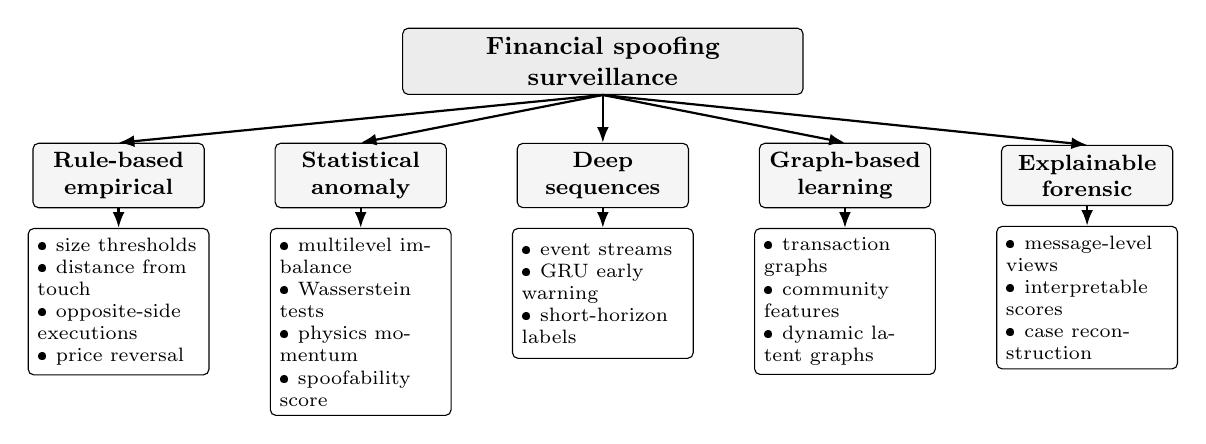
\begin{tikzpicture}[
        font=\scriptsize,
        root/.style={
            draw,
            rounded corners=2pt,
            fill=gray!15,
            align=center,
            text width=0.40\textwidth,
            minimum height=0.8cm,
            font=\small\bfseries
        },
        category/.style={
            draw,
            rounded corners=2pt,
            fill=gray!8,
            align=center,
            text width=0.16\textwidth,
            minimum height=0.75cm,
            font=\footnotesize\bfseries
        },
        detail/.style={
            draw,
            rounded corners=2pt,
            fill=white,
            align=left,
            text width=0.17\textwidth,
            minimum height=1.65cm
        },
        arrow/.style={-{Latex[length=2mm]}, thick}
    ]
        \node[root] (root) at (0,0) {Financial \mbox{spoofing} surveillance};

        \node[category] (rules) at (-6.15,-1.45) {Rule-based\\empirical};
        \node[category] (stat) at (-3.075,-1.45) {Statistical\\anomaly};
        \node[category] (seq) at (0,-1.45) {Deep\\sequences};
        \node[category] (graph) at (3.075,-1.45) {Graph-based\\learning};
        \node[category] (expl) at (6.15,-1.45) {Explainable\\forensic};

        \node[detail, below=0.25cm of rules] (rulesd) {\textbullet\ size thresholds\\\textbullet\ distance from touch\\\textbullet\ opposite-side executions\\\textbullet\ price reversal};
        \node[detail, below=0.25cm of stat] (statd) {\textbullet\ multilevel imbalance\\\textbullet\ Wasserstein tests\\\textbullet\ physics momentum\\\textbullet\ spoofability score};
        \node[detail, below=0.25cm of seq] (seqd) {\textbullet\ event streams\\\textbullet\ GRU early warning\\\textbullet\ short-horizon labels};
        \node[detail, below=0.25cm of graph] (graphd) {\textbullet\ transaction graphs\\\textbullet\ community features\\\textbullet\ dynamic latent graphs};
        \node[detail, below=0.25cm of expl] (expld) {\textbullet\ message-level views\\\textbullet\ interpretable scores\\\textbullet\ case reconstruction};

        \foreach \target in {rules,stat,seq,graph,expl} {
            \draw[arrow] (root.south) -- (\target.north);
        }
        \foreach \source/\target in {rules/rulesd,stat/statd,seq/seqd,graph/graphd,expl/expld} {
            \draw[arrow] (\source.south) -- (\target.north);
        }
    \end{tikzpicture}
    \caption{Method families in spoofing-detection research. The categories can overlap; each column identifies
    the main object or representation used by a strand of work.}
    \label{fig:method_taxonomy}
\end{figure}

Early empirical studies operationalize surveillance screens through interpretable order-book conditions. Using account-level
Korea Exchange data, \cite{LeeEomPark2013} identify large orders placed far from the best quote, followed by opposite-side trading and
subsequent withdrawal. Related surveillance rules have been applied to Brazilian equities
\cite{MendoncaDeGenaro2020}, FX spot markets \cite{StenforsSusai2021}, cross-market FX activity
\cite{StenforsEtAl2023}, and Taiwan derivatives \cite{ChenHsiehYang2026}. These studies connect a screen to observable
features such as order size, posting distance, cancellation timing, opposite-side execution, and short-lived price
impact. However, the reported implementations use venue-specific thresholds, and their reconstruction can require
privileged message data or account identifiers.

A second line of work monitors statistical anomalies in the order book. \cite{TaoDayLingDrapeau2022} derive spoofing
incentives from multilevel imbalance and propose a Wasserstein-distance statistic for real-time monitoring.
\cite{LiPolukarovaVentre2023} represent the order book with statistical-physics concepts and detect abnormal momentum in
cryptocurrency markets. Explainable forensic methods partly overlap with this family. Message-level visualization can
reconstruct prosecuted episodes \cite{DebieEtAl2023}. Interpretable probabilistic neural networks instead estimate how an
isolated limit order changes the conditional distribution of future prices and the expected gain from a hypothetical
manipulation strategy in centralized cryptocurrency markets \cite{FabreChallet2025}. The latter object measures
the \emph{spoofability} of an individual order; it does not establish whether one participant generated the candidate posture,
the smaller execution-side order, and the withdrawal. Our framework addresses this complementary attribution problem by
linking the observed actions through canonical actor keys while recording client or firm scope.

Machine-learning methods add temporal or relational structure. \cite{TuccellaNadlerSerban2021} formulate spoofing as an
early-warning problem and train a gated recurrent unit model on cryptocurrency order-book event streams. Graph methods move
the unit of analysis from isolated orders to networks of traders and transactions. This representation can
capture coordinated spoofing patterns \cite{KangMuNing2023,KangMuNing2024,XiangEtAl2025}. Reported models combine
temporal transaction graphs, community features, and dynamic latent representations. Their practical performance remains
difficult to compare because available labels, market settings, and validation designs differ.

These studies imply two requirements for the present surveillance setting. First, the features must retain their
microstructure interpretation. The screen must record candidate volume, posting distance from the touch, cancellation
timing, and the relation to an opposite-side execution. Second, any eventual validation must reflect scarce and noisy
enforcement labels, rare positive cases, and the analyst cost of false positives. Given the evidence currently available,
the model below preserves the auditability of rule-based surveillance while producing descriptive participant-attributed
order sequences from proprietary event data.

\section{Data}
\label{sec:data}

We use three CONSOB limit-order-book message samples. Risanamento covers June--November 2024, Nexi covers 23 April 2024,
and Ferrari covers 13 June 2024. The samples differ in duration and participant composition, so cross-instrument differences
are descriptive rather than controlled comparisons.

For an exploratory coverage audit, we also use an externally supplied CONSOB surveillance report containing $37$ alert
records supplied as positive seeds. These periods test whether the reconstruction covers reported activity; they are not
independently adjudicated manipulation labels. The source contains $35$ timed Ferrari records, one timed Nexi record, and
one Risanamento record that identifies only the trading date. We preserve every source record and merge timed intervals that
overlap or share an endpoint only within the same instrument and external subject. This yields $34$ distinct timed intervals;
the date-only Risanamento record remains outside the event-level denominator.

For timed records, we parse source bounds at millisecond precision and include both endpoints. We place raw events on a
common event-time axis using the first nonmissing timestamp in the priority order \texttt{TRADETIME}, \texttt{BOOKOUTTIME},
\texttt{BOOKIN}, and \texttt{SEQUENCETIME}. An execution is recovered when at least one constituent execution message lies
inside the closed union interval; its matched-withdrawal and strict-gate status are then read from event-level diagnostics.
The union interval, rather than each potentially overlapping source record, is the observational unit for timed counts.

We match each external subject in the identity namespace reported by the source. Consequently, an external firm can cover
several canonical actor keys when client identifiers are available internally. We therefore distinguish subject-scope overlap
from exact-actor correspondence and treat the latter as identifiable only when the external identity maps to one canonical
actor at the same granularity. The alert report contains no negative sample, so the comparison cannot estimate a
false-positive rate.

For each instrument, we reconstruct the visible order book from order-level events and infer tick size from reconstructed best
quotes. We compute resting-profile diagnostics over the first ten book ranks and separately construct the age-conditioned,
opposite-side candidate set. The main specification uses a $10$-second post-execution structural window, a $2$-second
rapid-withdrawal attribution window, a $2$-second reversion horizon measured from each assigned cancellation, and a maximum
candidate-order age of $90$ seconds.

The original client code is not available on every message. We therefore define one canonical actor key before constructing
events. If the original client code is present, it defines the actor; only when it is missing do we use the firm identifier.
The technical client value \texttt{0} is treated as missing rather than as an actor, so a message carrying this sentinel uses
the firm fallback when a firm identifier is available. The two namespaces are kept distinct, and every output records whether
attribution is at the client or firm level. Client-derived and firm-fallback keys are distinct canonical identities: the
fallback never merges a client-identified message with a firm-only message. Messages missing both identifiers are excluded
from actor-attributed analysis; none occurs in the reported samples. Firm fallback is coarser than client attribution and
can combine several clients represented by the same firm. It is therefore an identity fallback, not evidence that those
clients are one economic account.

Execution role is defined independently of actor identity. We retain individual execution messages marked exclusively passive or exclusively
aggressive and reject messages for which the two role flags are both set or both absent. Related execution messages are grouped into
one analytical execution when they share the trading partition---trading date, venue, market, instrument, and EMM code---as
well as canonical actor, order identifier, execution role, and side.

\pagebreak[4]

Passive executions also require a common resting price; aggressive executions can span several traded prices under the same order and sweep. Consecutive constituent execution
messages must be no more than $100$ milliseconds apart, with no intervening cancellation, modification, or new-order
lifecycle event for the same order. The $100$-millisecond threshold is operational, and reported findings are conditional on
it; sensitivity to alternative inter-execution-message gaps is not reported. Raw-message identifiers and the constituent
messages assigned to each execution remain available as provenance, while executions form the analytical unit for event
metrics and actor--partition aggregation. The resulting surveillance dossiers support analyst review and are not enforcement
labels.

\section{Model}
\label{sec:model}
The model translates the stylized contrast between market making and spoofing into observable sequence conditions. Its
central question is whether recent opposite-side orders disappear after the same participant executes. We therefore keep
three empirical components distinct. The complete top-$n$ resting profile supplies the descriptive DWI, SCI, and MSCI shape
diagnostics. The fixed, age-conditioned candidate set supplies matched-withdrawal quantities and WMSCI, which orders events
for review. The strict gate combines matching with prespecified conditions on withdrawal size, favorable movement, and reversion.
These are screening conditions, not estimates of causal influence or intent; the resting-profile, withdrawal, and
price-response quantities remain separate because they describe different parts of the mechanism.

% \subsection{Spoofer's timeline}
% \label{subsec:spoofing_timeline}
% \begin{enumerate}
%     \item The spoofer posts a large non bona fide order far away from the best quote and, simultaneously, a small bona 
%     fide order close to the best quote
%     \item The spoofer's small order gets executed due to the price move induced by the artificially increased volume
%     on the opposite side of the book
%     \item The spoofer cancels the large non bona fide order immediately after the execution
%     \begin{figure}[htbp]
%     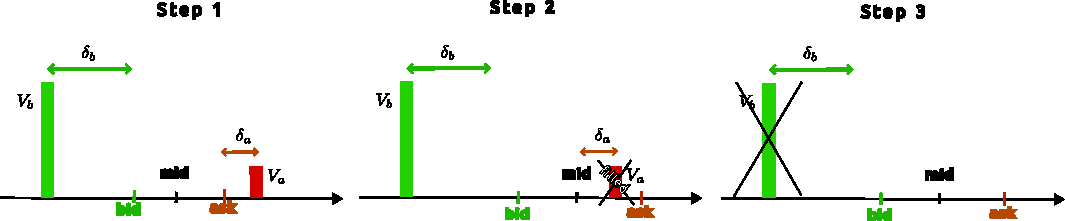
\includegraphics[width=\textwidth]{images/spoofer.pdf}
%     \caption{Timeline of a spoofing episode}
%     \end{figure}

% \end{enumerate}
% Let $i$ indicate the agent of interest, $V_a$ and $V_b$ represent the volumes of the agent's ask and bid orders, 
% respectively, and $\delta_a$ and $\delta_b$ represent their posting distances from the best quote. We consider 
% the following metric that we call distance-weighted imbalance:
% \begin{equation}
%     \left. \text{imb}_{t}^i = \frac{V_a \delta_a - V_b \delta_b}{V_a + V_b} \right|_i
% \end{equation}
% If we consider a sell intent for the spoofer, we expect $\text{imb}_{t}^i$ to be negative at step 1, to become more 
% negative at step 2, and to return to zero at step 3. The opposite holds for a buy intent.
% The crucial point is to distinguish this situation of imbalance between bid and ask from a rebalncing strategy of the market
% maker. In fact, a market maker can also post a large order on one side of the book and a small order on the other side, 
% but in this case we expect the large order to be close to the best quote and the small order to be far from the best 
% quote, while for a spoofer we seek for the opposite. Hence, in this case the imbalance would be positive and it would move
% towards zero more smoothly as the big order is executed, without a sharp and sudden jump as in the spoofer case.

\subsection{A Spatio-Temporal Framework for Spoofing Detection}
\label{sec:spoofer_timeline}

\Cref{fig:topn_spoofing_timeline} sketches the hypothesized sequence. The detector translates its states into observable
order, execution, and cancellation records rather than inferring the participant's purpose.

\begin{figure}[htbp]
    \centering
    \resizebox{0.95\textwidth}{!}{%
    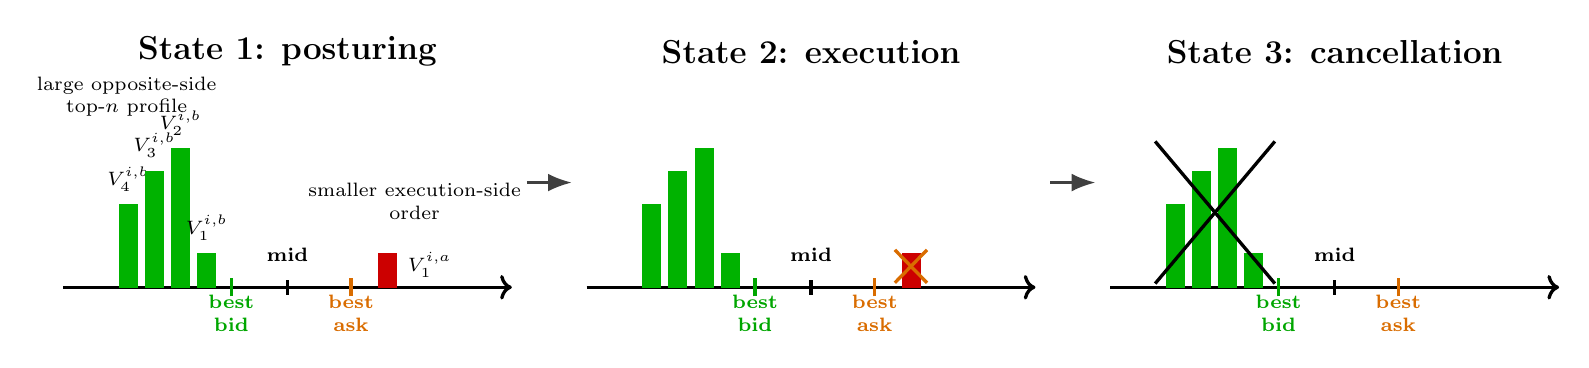
\begin{tikzpicture}[
        x=0.95cm,
        y=0.95cm,
        font=\small,
        book/.style={->, very thick},
        quote/.style={very thick},
        bid/.style={green!65!black},
        ask/.style={orange!85!black},
        fake/.style={fill=green!70!black, draw=green!70!black},
        real/.style={fill=red!80!black, draw=red!80!black},
        layer/.style={draw=black!45, fill=gray!8, rounded corners=2pt, minimum width=0.40cm},
        dist/.style={<->, black!70, very thick}
    ]
        \foreach \xshift/\step in {0/State 1: posturing,7.0/State 2: execution,14.0/State 3: cancellation} {
            \node[font=\large\bfseries] at (\xshift+3.0,3.15) {\step};
            \draw[book] (\xshift,0) -- (\xshift+6.0,0);
            \draw[quote,bid] (\xshift+2.25,-0.12) -- (\xshift+2.25,0.12)
                node[below=0.08cm, align=center, font=\scriptsize\bfseries] {best\\bid};
            \draw[quote] (\xshift+3.00,-0.10) -- (\xshift+3.00,0.10)
                node[above=0.10cm, font=\scriptsize\bfseries] {mid};
            \draw[quote,ask] (\xshift+3.85,-0.12) -- (\xshift+3.85,0.12)
                node[below=0.08cm, align=center, font=\scriptsize\bfseries] {best\\ask};
        }

        % State 1: layered bid-side deceptive profile and small ask-side bona fide order.
        \foreach \x/\h/\lab in {0.75/1.10/{$V^{i,b}_{4}$},1.10/1.55/{$V^{i,b}_{3}$},1.45/1.85/{$V^{i,b}_{2}$},1.80/0.45/{$V^{i,b}_{1}$}} {
            \draw[fake] (\x,0) rectangle +(0.24,\h);
            \node[above, font=\scriptsize] at (\x+0.12,\h+0.05) {\lab};
        }
        \draw[real] (4.22,0) rectangle +(0.24,0.45);
        \node[right, font=\scriptsize] at (4.48,0.30) {$V^{i,a}_{1}$};
        \node[align=center, font=\scriptsize] at (0.85,2.55) {large opposite-side\\top-$n$ profile};
        \node[align=center, font=\scriptsize] at (4.70,1.15) {smaller execution-side\\order};

        % State 2.
        \foreach \x/\h in {7.75/1.10,8.10/1.55,8.45/1.85,8.80/0.45} {
            \draw[fake] (\x,0) rectangle +(0.24,\h);
        }
        \draw[real] (11.22,0) rectangle +(0.24,0.45);
        \draw[orange!85!black, very thick] (11.12,0.06) -- (11.55,0.50);
        \draw[orange!85!black, very thick] (11.55,0.06) -- (11.12,0.50);


        % State 3.
        \foreach \x/\h in {14.75/1.10,15.10/1.55,15.45/1.85,15.80/0.45} {
            \draw[fake] (\x,0) rectangle +(0.24,\h);
        }
        \draw[black, very thick] (14.60,0.05) -- (16.20,1.95);
        \draw[black, very thick] (16.20,0.05) -- (14.60,1.95);


        \draw[-{Latex[length=3mm]}, thick, black!75] (6.2,1.4) -- (6.8,1.4);
        \draw[-{Latex[length=3mm]}, thick, black!75] (13.2,1.4) -- (13.8,1.4);
    \end{tikzpicture}%
    }
    \caption{Schematic top-$n$ timeline for the hypothesized spoofing mechanism. The large candidate posture forms \begin{review}a depth profile for the agent\end{review} over several bid levels, while the smaller order rests near the opposite best quote. The
    construction applies symmetrically to \begin{review}candidate episodes with buy or sell intent\end{review}. The figure shows the passive execution
    route; the operational reconstruction also admits an aggressive execution by the same actor.}
    \label{fig:topn_spoofing_timeline}
\end{figure}

The method represents a candidate episode as a conditional change in the participant's LOB footprint. A single order at
the best bid or ask does not capture this change. We instead use the participant's liquidity profile over the first $n$
price levels. This representation includes postures placed at Level 2, Level 3, or across adjacent levels, where displayed
liquidity can remain visible while facing less immediate execution risk.

\pagebreak[4]

The hypothesized mechanism for participant $i$ has three states:
\begin{enumerate}
    \item \textbf{State 1 (Candidate Posturing):} Shortly before the execution, the participant displays a large
    liquidity profile on one side of the book, typically away from the touch. An opposite-side execution anchors the
    operational reconstruction and may be passive or aggressive.
    \item \textbf{State 2 (Execution):} The large profile is present when the smaller opposite-side order executes. In the
    hypothesized mechanism, the profile can coincide with a more extreme measured imbalance before this execution.
    \item \textbf{State 3 (Withdrawal):} The participant rapidly cancels the opposite-side profile after the execution;
    under the stylized mechanism, this timing is consistent with reducing subsequent execution exposure.
\end{enumerate}

State 2 has two observable routes. In the passive route, the actor's resting order executes; in the aggressive route, the
actor initiates the trade against resting liquidity. Execution role changes how price and quantity are read and how messages
are grouped, but not actor identity. In both routes, the candidate posture is sought among the same actor's recent orders on
the side opposite to the execution. Neither an aggressive anchor nor a passive anchor identifies intent.

The three states motivate the reconstruction but do not define strict-set membership. For either execution route, the
candidate set contains same-actor, opposite-side orders observed in the top $10$ ranks before execution and satisfying the
$90$-second age limit. A cancellation within $2$ seconds provides matched-withdrawal evidence. The strict gate additionally
requires attributed withdrawal to exceed execution quantity and both midprice-response diagnostics to be positive. The
detector observes these conditions, not the participant's intent or the profile's causal effect on other traders. The recency
restriction prevents long-lived liquidity from entering a candidate episode solely because it was already resting in the book.

\subsubsection{\texorpdfstring{Top-$n$}{Top-n} Participant-Specific Depth Profiles}
\label{subsec:topn_depth_profiles}

We first define the participant-specific depth profile used throughout the model. Let $s \in \{b,a\}$ denote the bid or
ask side, and let $k=1,\ldots,n$ denote book rank. Rank $k=1$ is the best quote on side $s$, and
$V^{i,s}_{k}(t)$ is participant $i$'s displayed volume at time $t$ on that side and rank. The vector
\begin{equation}
    \mathbf{V}^{i,s}_{n}(t)
    = \left(V^{i,s}_{1}(t),\ldots,V^{i,s}_{n}(t)\right)
\end{equation}
collects these quantities over the first $n$ ranks. The vector preserves where liquidity is displayed rather than reducing
the participant's entire side of the book to one total. This distinction matters because a large order near the touch has
different execution risk from the same quantity posted at a deeper rank.

Raw displayed volume may not be comparable across assets or intraday periods with different market depth. The relative
profile therefore divides participant volume by total displayed market depth at the same side and rank:
\begin{equation}
    \widetilde V^{i,s}_{k}(t)
    =\begin{cases}
    \dfrac{V^{i,s}_{k}(t)}{D^{s}_{k}(t)},
    & D^{s}_{k}(t)>0,\\
    0,
    & D^{s}_{k}(t)=0,
    \end{cases}
    \label{eq:relative_agent_depth}
\end{equation}
where $D^{s}_{k}(t)$ is total displayed market depth on side $s$ and rank $k$. The zero-depth branch makes the rank-level
convention explicit; an imbalance remains undefined when the participant has no positive weighted footprint on either side.
We denote the distance from the touch by $d^{s}_{k}(t)$. In tick units, this distance equals the number of ticks between
rank $k$ and the same-side best quote, shifted upward by one. The shift gives Rank 1 a positive distance and preserves the
ordering of deeper ranks.

\subsubsection{Multilevel Distance-Weighted Imbalance}
\label{subsec:multilevel_dwi}

\paragraph{Economic intuition and a stylized parametric benchmark.}
We use a depth kernel to reduce the top-$n$ vector to a scalar weighted-liquidity measure. The kernel is designed to assign
high weight to ranks that remain represented in multilevel book data while facing comparatively low immediate execution
risk. The following parametric kernel illustrates this trade-off:
\begin{equation}
    \omega^{s,\mathrm{par}}_{k}(t)
    =
    \frac{
        e^{-\lambda d^{s}_{k}(t)}
        \left(1-e^{-\kappa d^{s}_{k}(t)}\right)
    }{
        \sum_{\ell=1}^{n}
        e^{-\lambda d^{s}_{\ell}(t)}\left(
        1-e^{-\kappa d^{s}_{\ell}(t)}\right)
    },
    \label{eq:depth_kernel}
\end{equation}
The visibility component $e^{-\lambda d}$ decreases with depth. The protection component
$1-e^{-\kappa d}$ increases as the displayed price moves away from immediate execution. Their product penalizes both the
high execution risk near the touch and the lower visibility deeper in the book. The parameters $\lambda$ and $\kappa$
control the two shapes. This expression is only a conceptual benchmark: the empirical analysis uses neither these weights
nor fitted values of $\lambda$ and $\kappa$. Instead, it constructs rank-level empirical proxies for each instrument and
book side.

\Cref{fig:depth_kernel_behavior} illustrates the benchmark trade-off and its discrete normalization; it is not an
estimated empirical profile.

\begin{figure}[htbp]
    \centering
    \resizebox{0.95\textwidth}{!}{%
    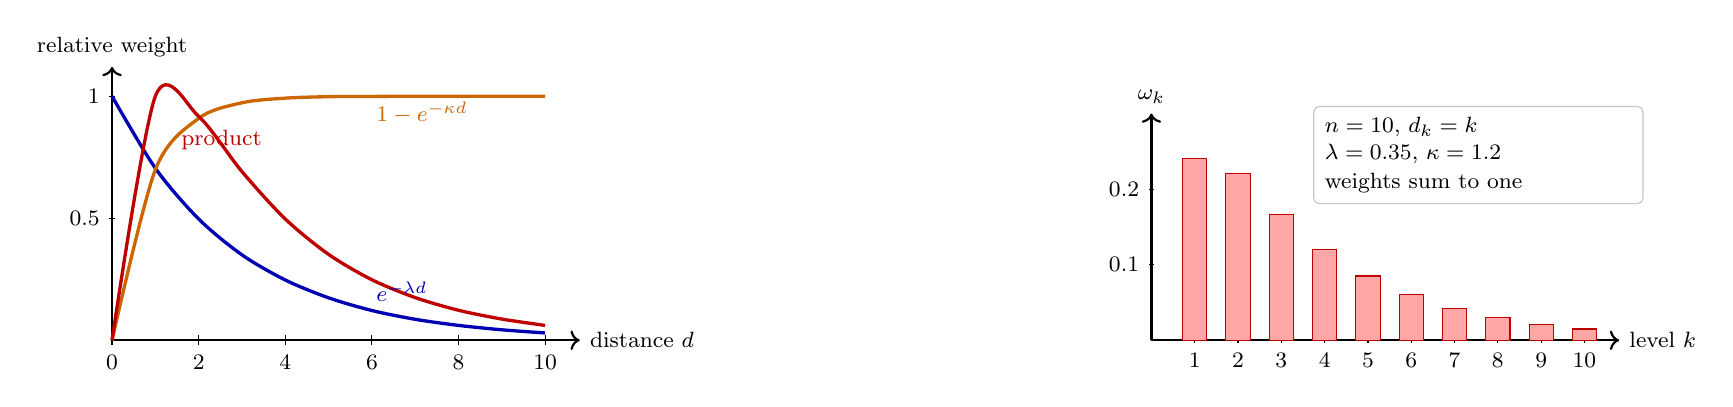
\begin{tikzpicture}[
        x=0.55cm,
        y=3.1cm,
        font=\footnotesize,
        axis/.style={->, thick},
        visibility/.style={very thick, blue!70!black},
        protection/.style={very thick, orange!80!black},
        kernel/.style={very thick, red!75!black},
        weightbar/.style={fill=red!35, draw=red!75!black},
        note/.style={draw=gray!45, rounded corners=2pt, fill=white, align=left, text width=3.9cm, inner sep=4pt}
    ]
        % Left panel: unnormalised ingredients, with the product rescaled to unit peak.
        \draw[axis] (0,0) -- (10.8,0) node[right] {distance $d$};
        \draw[axis] (0,0) -- (0,1.12) node[above, align=center] {relative weight};
        \foreach \x in {0,2,4,6,8,10} {
            \draw (\x,0.02) -- (\x,-0.02) node[below] {\x};
        }
        \foreach \y/\lab in {0.5/$0.5$,1/$1$} {
            \draw (0.06,\y) -- (-0.06,\y) node[left] {\lab};
        }

        \draw[visibility]
            plot[smooth] coordinates {(0,1.000) (1,0.705) (2,0.497) (3,0.350) (4,0.247) (5,0.174) (6,0.122) (7,0.086) (8,0.061) (9,0.043) (10,0.030)};
        \draw[protection]
            plot[smooth] coordinates {(0,0.000) (1,0.699) (2,0.909) (3,0.973) (4,0.992) (5,0.998) (6,0.999) (7,1.000) (8,1.000) (9,1.000) (10,1.000)};
        \draw[kernel]
            plot[smooth] coordinates {(0,0.000) (1,1.000) (2,0.917) (3,0.691) (4,0.497) (5,0.352) (6,0.248) (7,0.175) (8,0.123) (9,0.087) (10,0.061)};
        \node[visibility, anchor=west] at (5.85,0.20) {$e^{-\lambda d}$};
        \node[protection, anchor=west] at (5.85,0.93) {$1-e^{-\kappa d}$};
        \node[kernel, anchor=west] at (1.35,0.82) {product};

        % Right panel: discrete normalised top-n kernel weights.
        \begin{scope}[xshift=13.2cm, y=9.6cm]
            \draw[axis] (0,0) -- (10.8,0) node[right] {level $k$};
            \draw[axis] (0,0) -- (0,0.30) node[above] {$\omega_k$};
            \foreach \x in {1,2,3,4,5,6,7,8,9,10} {
                \draw (\x,0.004) -- (\x,-0.004) node[below] {\x};
            }
            \foreach \y/\lab in {0.1/$0.1$,0.2/$0.2$} {
                \draw (0.06,\y) -- (-0.06,\y) node[left] {\lab};
            }
            \foreach \x/\h in {1/0.241,2/0.221,3/0.166,4/0.120,5/0.085,6/0.060,7/0.042,8/0.030,9/0.021,10/0.015} {
                \draw[weightbar] (\x-0.28,0) rectangle (\x+0.28,\h);
            }
            \node[note] at (7.55,0.245)
            {$n=10$, $d_k=k$\\
            $\lambda=0.35$, $\kappa=1.2$\\[1pt]
            weights sum to one};
        \end{scope}
    \end{tikzpicture}%
    }
    \caption{Conceptual depth kernel in \cref{eq:depth_kernel}. The left panel shows decreasing visibility, increasing
    protection from immediate execution, and their product. The right panel shows normalized weights for one illustrative
    parameter choice. The empirical analysis uses the instrument- and side-specific kernel in
    \cref{eq:empirical_depth_kernel}, not these parametric weights.}
    \label{fig:depth_kernel_behavior}
\end{figure}

\paragraph{Operational empirical depth kernel.}
The operational kernel replaces both exponential components with rank-level empirical quantities. We calibrate each book
rank $k$ separately for instrument $m$ and side $s$. A rank receives more weight when its depth has a strong short-horizon
association with midprice changes and its displayed price is rarely reached over the same horizon. Tick distance can vary
for a given rank over time, but rank remains the calibrated unit.

\emph{Operational calculation.} We reconstruct a post-event top-$n$ snapshot after every ordered message. Let
$\mathcal{O}_{m,s,k}$ contain the snapshots in which rank $k$ exists on side $s$ and has positive displayed depth. For
each $t\in\mathcal{O}_{m,s,k}$, the indicator $R^{m,s}_{t,k}(H)$ equals one when at least one execution during $(t,t+H]$ occurs
at or through the rank's displayed price. An ask rank is reached when the maximum ask execution price in the window is at least
the displayed price. A bid rank is reached when the minimum bid execution price is at most the displayed price. We estimate
the rank-level message-snapshot hit frequency, denoted $\widehat p^{m,s}_{k}(H)$, from pooled hit and exposure counts:
\begin{equation}
    \widehat p^{m,s}_{k}(H)
    =
    \frac{
        \sum_{t\in\mathcal{O}_{m,s,k}}R^{m,s}_{t,k}(H)
    }{
        |\mathcal{O}_{m,s,k}|
    }.
    \label{eq:empirical_hit_probability}
\end{equation}
Each observable snapshot contributes once, even when the same rank appears at different tick distances. Thus,
\cref{eq:empirical_hit_probability} divides total hits by total exposures; it does not average distance-specific hit rates.
Realized tick distance is retained only as descriptive metadata and does not define additional kernel rows or enter a
parametric fit. The probability interpretation is conditional on message-snapshot sampling. The estimator is a short-horizon
proxy for whether the displayed price is reached, not an individual order's execution probability, which also depends on
queue position, order size, and intervening cancellations.
We define the protection component as the complement of the hit probability:
\begin{equation}
    \widehat\rho^{m,s}_{k}(H)=1-\widehat p^{m,s}_{k}(H),
    \label{eq:empirical_protection_profile}
\end{equation}
A value of $\widehat\rho^{m,s}_{k}(H)$ near one indicates that rank $k$ is rarely reached over horizon $H$.

The second component measures the association between displayed depth and subsequent short-horizon price changes. Let
$D^{m,s}_{k}(t)$ denote total market depth, rather than participant-$i$ depth, at rank $k$. Total displayed top-$n$ depth at
snapshot $t$ is
\begin{equation}
    D^{m}_{n}(t)
    =
    \sum_{r=1}^{n}\left(D^{m,a}_{r}(t)+D^{m,b}_{r}(t)\right).
    \label{eq:total_topn_market_depth}
\end{equation}
We then define the signed and normalized contribution of side $s$ and rank $k$:
\begin{equation}
    Z^{m,s}_{t,k}
    =
    \sigma_s\frac{D^{m,s}_{k}(t)}{D^{m}_{n}(t)},
    \qquad
    \sigma_s= \begin{cases}
        +1, & s=ask,\\
        -1, & s=bid.
    \end{cases}
    \label{eq:normalized_level_contribution}
\end{equation}
The magnitude $|Z^{m,s}_{t,k}|$ is the fraction of visible top-$n$ depth supplied by that side and rank. The sign makes ask
and bid depth contribute in opposite directions to imbalance.

For each snapshot, $M^m_{t,H}$ is the last finite reconstructed midprice observed after $t$ and no later than $t+H$.
The corresponding price change is $\Delta M^m_{t,H}=M^m_{t,H}-M^m(t)$. Let $\mathcal{V}_{m,s,k}(H)$ contain the rank-$k$
snapshots for which both midprices are finite. For each instrument--side--rank cell, we compute the following pooled
empirical covariance in absolute value, normalized by the number of eligible snapshots. The overbars denote sample means over
$\mathcal{V}_{m,s,k}(H)$:
\begin{equation}
    \widehat\nu^{m,s}_{k}(H)
    =
    \left|
        \frac{1}{|\mathcal{V}_{m,s,k}(H)|}
        \sum_{t\in\mathcal{V}_{m,s,k}(H)}
        \left(Z^{m,s}_{t,k}-\overline Z^{m,s}_{k}\right)
        \left(\Delta M^m_{t,H}-\overline{\Delta M}^{m,s}_{k,H}\right)
    \right|.
    \label{eq:empirical_visibility_covariance}
\end{equation}
The absolute value makes $\widehat\nu^{m,s}_{k}(H)$ a measure of magnitude, rather than direction, of rank-specific
co-movement. We pool observations across realized tick distances before computing the covariance and do not compute or
average separate distance-bucket covariances. This quantity is a weighting proxy, not a causal estimate of price impact.
It is expressed in the instrument's price units, so it allocates weights only across ranks on the same side of one
instrument and does not support cross-instrument covariance comparisons.

The empirical kernel follows the same multiplicative decomposition as \cref{eq:depth_kernel}, but no exponential curve is
fitted. Before normalization, we enforce a zero lower bound on protection and apply a named $10^{-12}$ numerical floor to
the absolute covariance:
\begin{equation}
    \widetilde\rho^{m,s}_{k}(H)=\max\{1-\widehat p^{m,s}_{k}(H),0\},
    \qquad
    \widetilde\nu^{m,s}_{k}(H)=\max\{\widehat\nu^{m,s}_{k}(H),10^{-12}\},
    \label{eq:empirical_kernel_floors}
\end{equation}
We normalize the product of these two quantities within each instrument and side:
\begin{equation}
    \widehat\omega^{m,s}_{k}(H)
    =
    \frac{
        \widetilde\nu^{m,s}_{k}(H)\,\widetilde\rho^{m,s}_{k}(H)
    }{
        \sum_{\ell=1}^{n}\widetilde\nu^{m,s}_{\ell}(H)\,\widetilde\rho^{m,s}_{\ell}(H)
    }.
    \label{eq:empirical_depth_kernel}
\end{equation}
The denominator must be finite and strictly positive. If every rank on a side has zero protection, or if the product is
otherwise degenerate, calibration fails instead of returning an uninterpretable all-zero vector. The covariance floor is a
numerical regularizer rather than empirical evidence of price association. When estimated covariances are at or below the
floor, relative weights can be driven primarily by protection and must not be interpreted as evidence of a rank-specific
price association. Every reported kernel in \cref{tab:empirical_depth_kernel_calibration} passes the normalization condition and
sums to one before rounding.

In the remaining formulas, we use the shorthand
$\omega^{s}_{k}(t)\equiv\widehat\omega^{m,s}_{k}(H)$ for an event in instrument $m$; the time argument indicates that the
fixed weight is applied to a time-varying profile. Every event for instrument $m$ uses the same calibrated kernel. The kernel is not
re-estimated by actor, event, or observed outcome, and calibration admits only one weight for each $(m,s,k)$ cell. The
descriptive analysis uses the full available sample for each instrument. A prospective or out-of-sample application must
instead estimate the kernel on an earlier training period and hold it fixed, so that future order flow does not enter the
weights.

\begin{table}[htbp]
\centering
\caption{Empirical top-$10$ depth-kernel weights estimated on the full sample at horizon $H=10$ seconds. Values are rounded to
three decimal places and sum to one within each instrument and side before rounding. These weights, rather than fitted
exponential parameters, enter the empirical spoofing metrics.}
\label{tab:empirical_depth_kernel_calibration}
\scriptsize
\setlength{\tabcolsep}{1.7pt}
\begin{tabular}{ll*{10}{r}}
\toprule
Instrument & Side & $\widehat\omega_1$ & $\widehat\omega_2$ & $\widehat\omega_3$ & $\widehat\omega_4$ & $\widehat\omega_5$ & $\widehat\omega_6$ & $\widehat\omega_7$ & $\widehat\omega_8$ & $\widehat\omega_9$ & $\widehat\omega_{10}$ \\
\midrule
Risanamento & Ask & 0.127 & 0.248 & 0.348 & 0.062 & 0.004 & 0.039 & 0.018 & 0.012 & 0.078 & 0.064 \\
             & Bid & 0.526 & 0.012 & 0.019 & 0.146 & 0.091 & 0.065 & 0.082 & 0.034 & 0.002 & 0.024 \\
Nexi        & Ask & 0.028 & 0.069 & 0.033 & 0.138 & 0.225 & 0.149 & 0.275 & 0.011 & 0.020 & 0.051 \\
             & Bid & 0.045 & 0.166 & 0.184 & 0.276 & 0.165 & 0.033 & 0.006 & 0.052 & 0.064 & 0.008 \\
Ferrari     & Ask & 0.095 & 0.022 & 0.016 & 0.209 & 0.270 & 0.032 & 0.144 & 0.032 & 0.033 & 0.147 \\
             & Bid & 0.148 & 0.107 & 0.007 & 0.054 & 0.072 & 0.197 & 0.102 & 0.038 & 0.176 & 0.100 \\
\bottomrule
\end{tabular}
\end{table}

The operational calibration uses the first ten ranks and the same $H=10$ second horizon for every instrument. It produces
20 weights per instrument, one for each side--rank combination. The kernel remains side-specific. To draw one curve per
instrument for visualization only, we average the bid and ask weights at each rank:
\begin{equation}
    \overline{\omega}^{m}_{k}(H)
    =
    \frac{1}{2}\left(
        \widehat\omega^{m,a}_{k}(H)
        +
        \widehat\omega^{m,b}_{k}(H)
    \right).
    \label{eq:side_averaged_empirical_kernel}
\end{equation}
Each side-specific kernel sums to one, so $\sum_{k=1}^{10}\overline{\omega}^{m}_{k}(H)=1$. We use this average only in
\cref{fig:empirical_top10_kernel_profiles}. The empirical surveillance metrics use the side-specific top-$10$ weights in
\cref{tab:empirical_depth_kernel_calibration}.

\begin{figure}[htbp]
    \centering
    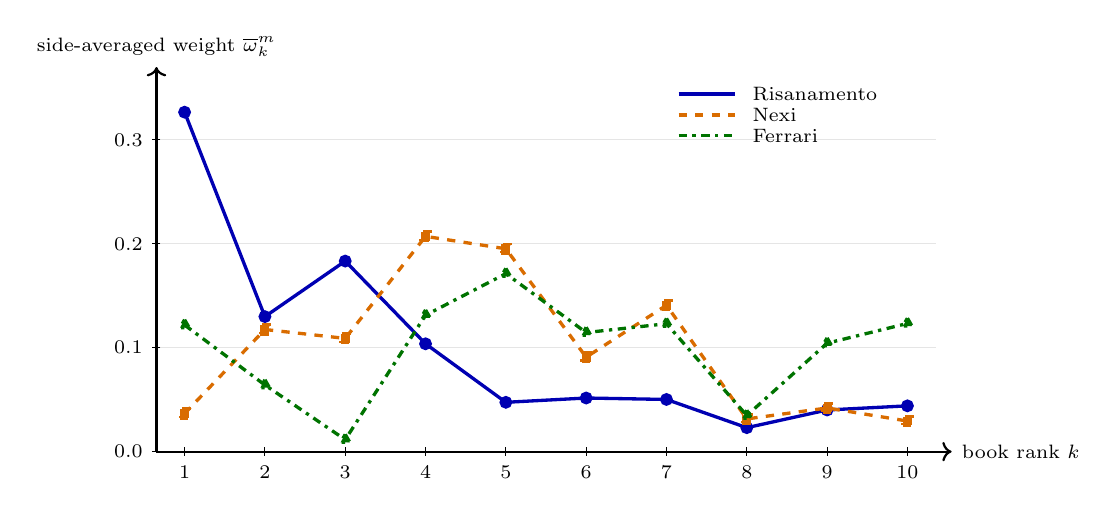
\begin{tikzpicture}[
        x=1.02cm,
        y=13.2cm,
        font=\scriptsize,
        axis/.style={->, thick},
        grid/.style={gray!20, thin},
        risanamento/.style={blue!70!black, very thick, mark=*, mark size=1.7pt},
        nexi/.style={orange!85!black, very thick, dashed, mark=square*, mark size=1.6pt},
        ferrari/.style={green!45!black, very thick, dash dot, mark=triangle*, mark size=1.9pt}
    ]
        \foreach \y in {0.1,0.2,0.3} {
            \draw[grid] (0.65,\y) -- (10.35,\y);
        }
        \draw[axis] (0.65,0) -- (10.55,0) node[right] {book rank $k$};
        \draw[axis] (0.65,0) -- (0.65,0.37) node[above, align=center]
            {side-averaged weight $\overline{\omega}^{m}_{k}$};

        \foreach \x in {1,...,10} {
            \draw (\x,0.004) -- (\x,-0.004) node[below] {\x};
        }
        \foreach \y/\lab in {0.0/$0.0$,0.1/$0.1$,0.2/$0.2$,0.3/$0.3$} {
            \draw (0.70,\y) -- (0.60,\y) node[left] {\lab};
        }

        \draw[risanamento]
            plot coordinates {
                (1,0.326590) (2,0.129904) (3,0.183346) (4,0.103747) (5,0.047449)
                (6,0.051590) (7,0.050207) (8,0.023040) (9,0.040075) (10,0.044052)
            };
        \draw[nexi]
            plot coordinates {
                (1,0.036660) (2,0.117508) (3,0.108946) (4,0.207104) (5,0.195161)
                (6,0.090903) (7,0.140818) (8,0.031470) (9,0.042001) (10,0.029429)
            };
        \draw[ferrari]
            plot coordinates {
                (1,0.121867) (2,0.064095) (3,0.011556) (4,0.131256) (5,0.171245)
                (6,0.114549) (7,0.123072) (8,0.034722) (9,0.104320) (10,0.123319)
            };

        \draw[risanamento] (7.15,0.344) -- (7.85,0.344);
        \node[anchor=west] at (7.95,0.344) {Risanamento};
        \draw[nexi] (7.15,0.324) -- (7.85,0.324);
        \node[anchor=west] at (7.95,0.324) {Nexi};
        \draw[ferrari] (7.15,0.304) -- (7.85,0.304);
        \node[anchor=west] at (7.95,0.304) {Ferrari};
    \end{tikzpicture}
    \caption{Empirical top-$10$ depth-kernel profiles estimated on the full sample at $H=10$ seconds. Each line is the arithmetic mean of
    the separately normalized bid and ask weights in \cref{eq:side_averaged_empirical_kernel}. The mean permits one curve
    per instrument on a common rank axis and is used only for visualization. Surveillance metrics use the underlying
    side-specific kernels.}
    \label{fig:empirical_top10_kernel_profiles}
\end{figure}
\FloatBarrier

To expose the two empirical inputs rather than only their normalized product,
\Cref{fig:empirical_topn_visibility_profiles,fig:empirical_topn_execution_risk_profiles} plot the side-specific visibility
and execution-risk profiles used in the calibration. The second plot reports
$\widehat p^{m,s}_{k}(H)$ directly; the
kernel uses its protection complement $\widehat\rho^{m,s}_{k}(H)=1-\widehat p^{m,s}_{k}(H)$.

% Generated by scripts/generate_empirical_kernel_component_figures.py; do not edit manually.
% calibration root: outputs/depth_kernel_calibration/20260717_145624_rank_pooled_top10_h10
% source RISANAMENTO: outputs/depth_kernel_calibration/20260717_145624_rank_pooled_top10_h10/RISANAMENTO_top10_h10/empirical_depth_kernel.csv sha256=6ecb2071cf524f6090dff6596dc64248cbf59af2c55cf0d33e0649fcc52abe45
% source NEXI: outputs/depth_kernel_calibration/20260717_145624_rank_pooled_top10_h10/NEXI_top10_h10/empirical_depth_kernel.csv sha256=deaeb5a1c7a301d48c51347fbc4bdc2dc389281302aeb41192c20190920335f5
% source FERRARI: outputs/depth_kernel_calibration/20260717_145624_rank_pooled_top10_h10/FERRARI_top10_h10/empirical_depth_kernel.csv sha256=d5fdc562b059874471a511f2990341ceed08f434ddefb8b3cf31589979a67540

% data column: visibility_component
\begin{figure}[!ht]
\centering
\resizebox{\textwidth}{!}{%
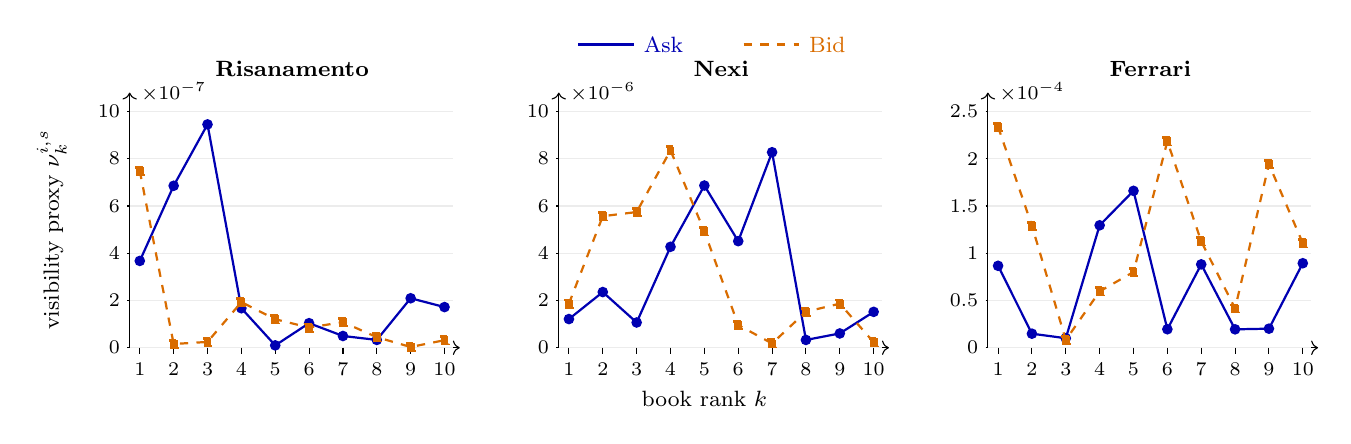
\begin{tikzpicture}
\begin{scope}[xshift=0.00cm]
\begin{scope}[x=0.43cm,y=0.30000000cm]
  \draw[->] (0.7,0) -- (10.45,0);
  \draw[->] (0.7,0) -- (0.7,10.8);
  \draw[gray!15] (0.7,0) -- (10.25,0);
  \draw (0.63,0) -- (0.7,0) node[left,font=\scriptsize] {0};
  \draw[gray!15] (0.7,2) -- (10.25,2);
  \draw (0.63,2) -- (0.7,2) node[left,font=\scriptsize] {2};
  \draw[gray!15] (0.7,4) -- (10.25,4);
  \draw (0.63,4) -- (0.7,4) node[left,font=\scriptsize] {4};
  \draw[gray!15] (0.7,6) -- (10.25,6);
  \draw (0.63,6) -- (0.7,6) node[left,font=\scriptsize] {6};
  \draw[gray!15] (0.7,8) -- (10.25,8);
  \draw (0.63,8) -- (0.7,8) node[left,font=\scriptsize] {8};
  \draw[gray!15] (0.7,10) -- (10.25,10);
  \draw (0.63,10) -- (0.7,10) node[left,font=\scriptsize] {10};
  \draw (1,0) -- (1,-0.025 * 10) node[below,font=\scriptsize] {1};
  \draw (2,0) -- (2,-0.025 * 10) node[below,font=\scriptsize] {2};
  \draw (3,0) -- (3,-0.025 * 10) node[below,font=\scriptsize] {3};
  \draw (4,0) -- (4,-0.025 * 10) node[below,font=\scriptsize] {4};
  \draw (5,0) -- (5,-0.025 * 10) node[below,font=\scriptsize] {5};
  \draw (6,0) -- (6,-0.025 * 10) node[below,font=\scriptsize] {6};
  \draw (7,0) -- (7,-0.025 * 10) node[below,font=\scriptsize] {7};
  \draw (8,0) -- (8,-0.025 * 10) node[below,font=\scriptsize] {8};
  \draw (9,0) -- (9,-0.025 * 10) node[below,font=\scriptsize] {9};
  \draw (10,0) -- (10,-0.025 * 10) node[below,font=\scriptsize] {10};
  \node[anchor=south west,font=\scriptsize] at (0.75,10) {$\times 10^{-7}$};
  \node[rotate=90,font=\footnotesize] at (-1.6,5) {visibility proxy $\nu_k^{i,s}$};
  \node[font=\footnotesize\bfseries] at (5.5,11.8) {Risanamento};
  \draw[blue!70!black, thick, mark=*, mark size=1.5pt] plot coordinates {(1,3.675229767983178) (2,6.855802152861837) (3,9.454395390358135) (4,1.6711452429542564) (5,0.09967103872544607) (6,1.03986078936913) (7,0.49722130939049286) (8,0.331027311346062) (9,2.094561089973038) (10,1.7209334991488594)};
  % RISANAMENTO ask visibility_component raw: 1:3.6752297679831775e-07, 2:6.855802152861836e-07, 3:9.4543953903581345e-07, 4:1.6711452429542563e-07, 5:9.9671038725446058e-09, 6:1.03986078936913e-07, 7:4.9722130939049281e-08, 8:3.31027311346062e-08, 9:2.0945610899730381e-07, 10:1.7209334991488592e-07
  \draw[orange!85!black, thick, dashed, mark=square*, mark size=1.4pt] plot coordinates {(1,7.4850054933810215) (2,0.15725764971410325) (3,0.24659322933232064) (4,1.930205433978854) (5,1.2069432758813796) (6,0.8540517059063696) (7,1.0836250920231838) (8,0.4466903180509029) (9,0.031098089940439774) (10,0.31967530278917544)};
  % RISANAMENTO bid visibility_component raw: 1:7.4850054933810209e-07, 2:1.5725764971410324e-08, 3:2.4659322933232062e-08, 4:1.9302054339788539e-07, 5:1.2069432758813797e-07, 6:8.5405170590636958e-08, 7:1.0836250920231838e-07, 8:4.4669031805090292e-08, 9:3.1098089940439771e-09, 10:3.1967530278917541e-08
\end{scope}
\end{scope}
\begin{scope}[xshift=5.45cm]
\begin{scope}[x=0.43cm,y=0.30000000cm]
  \draw[->] (0.7,0) -- (10.45,0);
  \draw[->] (0.7,0) -- (0.7,10.8);
  \draw[gray!15] (0.7,0) -- (10.25,0);
  \draw (0.63,0) -- (0.7,0) node[left,font=\scriptsize] {0};
  \draw[gray!15] (0.7,2) -- (10.25,2);
  \draw (0.63,2) -- (0.7,2) node[left,font=\scriptsize] {2};
  \draw[gray!15] (0.7,4) -- (10.25,4);
  \draw (0.63,4) -- (0.7,4) node[left,font=\scriptsize] {4};
  \draw[gray!15] (0.7,6) -- (10.25,6);
  \draw (0.63,6) -- (0.7,6) node[left,font=\scriptsize] {6};
  \draw[gray!15] (0.7,8) -- (10.25,8);
  \draw (0.63,8) -- (0.7,8) node[left,font=\scriptsize] {8};
  \draw[gray!15] (0.7,10) -- (10.25,10);
  \draw (0.63,10) -- (0.7,10) node[left,font=\scriptsize] {10};
  \draw (1,0) -- (1,-0.025 * 10) node[below,font=\scriptsize] {1};
  \draw (2,0) -- (2,-0.025 * 10) node[below,font=\scriptsize] {2};
  \draw (3,0) -- (3,-0.025 * 10) node[below,font=\scriptsize] {3};
  \draw (4,0) -- (4,-0.025 * 10) node[below,font=\scriptsize] {4};
  \draw (5,0) -- (5,-0.025 * 10) node[below,font=\scriptsize] {5};
  \draw (6,0) -- (6,-0.025 * 10) node[below,font=\scriptsize] {6};
  \draw (7,0) -- (7,-0.025 * 10) node[below,font=\scriptsize] {7};
  \draw (8,0) -- (8,-0.025 * 10) node[below,font=\scriptsize] {8};
  \draw (9,0) -- (9,-0.025 * 10) node[below,font=\scriptsize] {9};
  \draw (10,0) -- (10,-0.025 * 10) node[below,font=\scriptsize] {10};
  \node[anchor=south west,font=\scriptsize] at (0.75,10) {$\times 10^{-6}$};
  \node[font=\footnotesize\bfseries] at (5.5,11.8) {Nexi};
  \draw[blue!70!black, thick, mark=*, mark size=1.5pt] plot coordinates {(1,1.2138032154980023) (2,2.357195510456608) (3,1.0685006264223715) (4,4.273217243409157) (5,6.866026041374058) (6,4.512030446576142) (7,8.275878917434618) (8,0.32997233355025435) (9,0.6049414509297961) (10,1.5188249155682871)};
  % NEXI ask visibility_component raw: 1:1.2138032154980023e-06, 2:2.357195510456608e-06, 3:1.0685006264223715e-06, 4:4.2732172434091567e-06, 5:6.8660260413740573e-06, 6:4.5120304465761415e-06, 7:8.2758789174346172e-06, 8:3.2997233355025434e-07, 9:6.0494145092979615e-07, 10:1.5188249155682871e-06
  \draw[orange!85!black, thick, dashed, mark=square*, mark size=1.4pt] plot coordinates {(1,1.8674773855957816) (2,5.568884213770531) (3,5.7442838166896815) (4,8.353844420062963) (5,4.925771459538285) (6,0.9619962140487628) (7,0.1805094913160257) (8,1.5237267589959187) (9,1.8662709068477343) (10,0.2317283350241909)};
  % NEXI bid visibility_component raw: 1:1.8674773855957815e-06, 2:5.5688842137705302e-06, 3:5.7442838166896813e-06, 4:8.3538444200629627e-06, 5:4.9257714595382846e-06, 6:9.6199621404876272e-07, 7:1.8050949131602569e-07, 8:1.5237267589959187e-06, 9:1.8662709068477342e-06, 10:2.3172833502419091e-07
\end{scope}
\end{scope}
\begin{scope}[xshift=10.90cm]
\begin{scope}[x=0.43cm,y=1.20000000cm]
  \draw[->] (0.7,0) -- (10.45,0);
  \draw[->] (0.7,0) -- (0.7,2.7);
  \draw[gray!15] (0.7,0) -- (10.25,0);
  \draw (0.63,0) -- (0.7,0) node[left,font=\scriptsize] {0};
  \draw[gray!15] (0.7,0.5) -- (10.25,0.5);
  \draw (0.63,0.5) -- (0.7,0.5) node[left,font=\scriptsize] {0.5};
  \draw[gray!15] (0.7,1) -- (10.25,1);
  \draw (0.63,1) -- (0.7,1) node[left,font=\scriptsize] {1};
  \draw[gray!15] (0.7,1.5) -- (10.25,1.5);
  \draw (0.63,1.5) -- (0.7,1.5) node[left,font=\scriptsize] {1.5};
  \draw[gray!15] (0.7,2) -- (10.25,2);
  \draw (0.63,2) -- (0.7,2) node[left,font=\scriptsize] {2};
  \draw[gray!15] (0.7,2.5) -- (10.25,2.5);
  \draw (0.63,2.5) -- (0.7,2.5) node[left,font=\scriptsize] {2.5};
  \draw (1,0) -- (1,-0.025 * 2.5) node[below,font=\scriptsize] {1};
  \draw (2,0) -- (2,-0.025 * 2.5) node[below,font=\scriptsize] {2};
  \draw (3,0) -- (3,-0.025 * 2.5) node[below,font=\scriptsize] {3};
  \draw (4,0) -- (4,-0.025 * 2.5) node[below,font=\scriptsize] {4};
  \draw (5,0) -- (5,-0.025 * 2.5) node[below,font=\scriptsize] {5};
  \draw (6,0) -- (6,-0.025 * 2.5) node[below,font=\scriptsize] {6};
  \draw (7,0) -- (7,-0.025 * 2.5) node[below,font=\scriptsize] {7};
  \draw (8,0) -- (8,-0.025 * 2.5) node[below,font=\scriptsize] {8};
  \draw (9,0) -- (9,-0.025 * 2.5) node[below,font=\scriptsize] {9};
  \draw (10,0) -- (10,-0.025 * 2.5) node[below,font=\scriptsize] {10};
  \node[anchor=south west,font=\scriptsize] at (0.75,2.5) {$\times 10^{-4}$};
  \node[font=\footnotesize\bfseries] at (5.5,2.95) {Ferrari};
  \draw[blue!70!black, thick, mark=*, mark size=1.5pt] plot coordinates {(1,0.8669505020816368) (2,0.1485759198632677) (3,0.10059702674753057) (4,1.2956601892544413) (5,1.6603869526647457) (6,0.19557846353831482) (7,0.8821362998985953) (8,0.19476684019606572) (9,0.20169455861968041) (10,0.8943935007246941)};
  % FERRARI ask visibility_component raw: 1:8.6695050208163686e-05, 2:1.485759198632677e-05, 3:1.0059702674753058e-05, 4:0.00012956601892544412, 5:0.00016603869526647457, 6:1.9557846353831483e-05, 7:8.8213629989859532e-05, 8:1.9476684019606572e-05, 9:2.0169455861968043e-05, 10:8.9439350072469421e-05
  \draw[orange!85!black, thick, dashed, mark=square*, mark size=1.4pt] plot coordinates {(1,2.338679183565612) (2,1.291355118638466) (3,0.08201799287649617) (4,0.5966462138610819) (5,0.8015132512207448) (6,2.184977047983166) (7,1.1257505456756975) (8,0.41537003587522076) (9,1.9429973087449643) (10,1.1061392811485924)};
  % FERRARI bid visibility_component raw: 1:0.0002338679183565612, 2:0.00012913551186384661, 3:8.2017992876496163e-06, 4:5.9664621386108187e-05, 5:8.0151325122074484e-05, 6:0.00021849770479831661, 7:0.00011257505456756977, 8:4.1537003587522077e-05, 9:0.00019429973087449644, 10:0.00011061392811485925
\end{scope}
\end{scope}
\node[font=\footnotesize] at (7.6,-0.65) {book rank $k$};
\draw[blue!70!black,thick,mark=*,mark size=1.5pt] (6.0,3.85) -- (6.7,3.85) node[right,font=\footnotesize] {Ask};
\draw[orange!85!black,thick,dashed,mark=square*,mark size=1.4pt] (8.1,3.85) -- (8.8,3.85) node[right,font=\footnotesize] {Bid};
\end{tikzpicture}%
}
\caption{Side-specific empirical visibility proxy by book rank. Each panel shows the stored \texttt{visibility\_component} values from the full-sample top-$10$, $h=10$-second calibration. Separate axis multipliers preserve the instrument-specific price units; vertical magnitudes should not be compared across instruments.}
\label{fig:empirical_topn_visibility_profiles}
\end{figure}

% data column: hit_probability; protection_component = 1 - hit_probability
\begin{figure}[!ht]
\centering
\resizebox{\textwidth}{!}{%
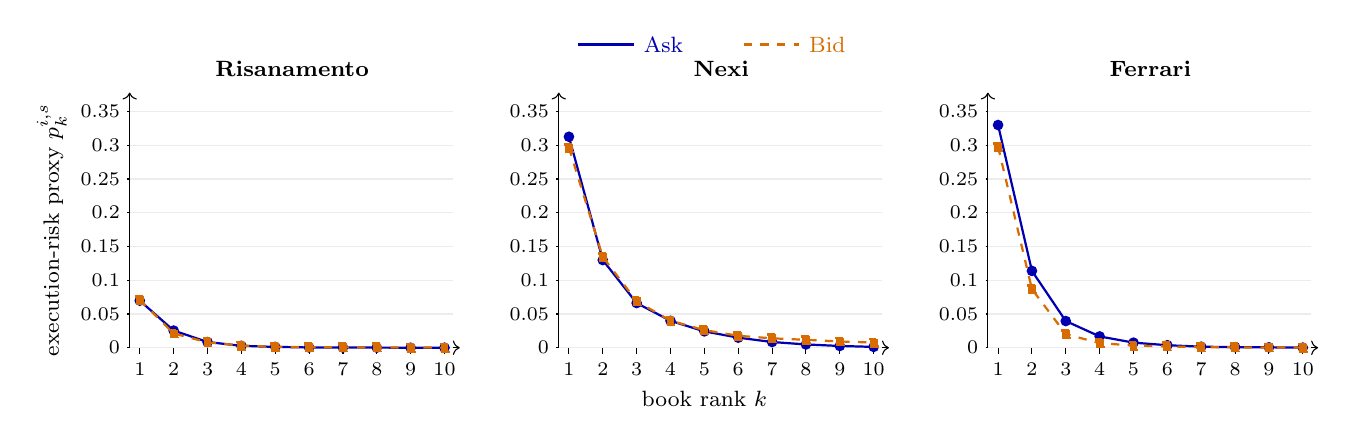
\begin{tikzpicture}
\begin{scope}[xshift=0.00cm]
\begin{scope}[x=0.43cm,y=8.57142857cm]
  \draw[->] (0.7,0) -- (10.45,0);
  \draw[->] (0.7,0) -- (0.7,0.378);
  \draw[gray!15] (0.7,0) -- (10.25,0);
  \draw (0.63,0) -- (0.7,0) node[left,font=\scriptsize] {0};
  \draw[gray!15] (0.7,0.05) -- (10.25,0.05);
  \draw (0.63,0.05) -- (0.7,0.05) node[left,font=\scriptsize] {0.05};
  \draw[gray!15] (0.7,0.1) -- (10.25,0.1);
  \draw (0.63,0.1) -- (0.7,0.1) node[left,font=\scriptsize] {0.1};
  \draw[gray!15] (0.7,0.15) -- (10.25,0.15);
  \draw (0.63,0.15) -- (0.7,0.15) node[left,font=\scriptsize] {0.15};
  \draw[gray!15] (0.7,0.2) -- (10.25,0.2);
  \draw (0.63,0.2) -- (0.7,0.2) node[left,font=\scriptsize] {0.2};
  \draw[gray!15] (0.7,0.25) -- (10.25,0.25);
  \draw (0.63,0.25) -- (0.7,0.25) node[left,font=\scriptsize] {0.25};
  \draw[gray!15] (0.7,0.3) -- (10.25,0.3);
  \draw (0.63,0.3) -- (0.7,0.3) node[left,font=\scriptsize] {0.3};
  \draw[gray!15] (0.7,0.35) -- (10.25,0.35);
  \draw (0.63,0.35) -- (0.7,0.35) node[left,font=\scriptsize] {0.35};
  \draw (1,0) -- (1,-0.025 * 0.35) node[below,font=\scriptsize] {1};
  \draw (2,0) -- (2,-0.025 * 0.35) node[below,font=\scriptsize] {2};
  \draw (3,0) -- (3,-0.025 * 0.35) node[below,font=\scriptsize] {3};
  \draw (4,0) -- (4,-0.025 * 0.35) node[below,font=\scriptsize] {4};
  \draw (5,0) -- (5,-0.025 * 0.35) node[below,font=\scriptsize] {5};
  \draw (6,0) -- (6,-0.025 * 0.35) node[below,font=\scriptsize] {6};
  \draw (7,0) -- (7,-0.025 * 0.35) node[below,font=\scriptsize] {7};
  \draw (8,0) -- (8,-0.025 * 0.35) node[below,font=\scriptsize] {8};
  \draw (9,0) -- (9,-0.025 * 0.35) node[below,font=\scriptsize] {9};
  \draw (10,0) -- (10,-0.025 * 0.35) node[below,font=\scriptsize] {10};
  \node[rotate=90,font=\footnotesize] at (-1.6,0.175) {execution-risk proxy $p_k^{i,s}$};
  \node[font=\footnotesize\bfseries] at (5.5,0.413) {Risanamento};
  \draw[blue!70!black, thick, mark=*, mark size=1.5pt] plot coordinates {(1,0.06972349940165018) (2,0.02545533573561784) (3,0.008478028770510227) (4,0.0028297304716921367) (5,0.0012412635498727) (6,0.0004097636793952453) (7,0.0002830315509421413) (8,0.00021971635327554557) (9,0.0) (10,0.0)};
  % RISANAMENTO ask hit_probability raw: 1:0.06972349940165018, 2:0.02545533573561784, 3:0.0084780287705102271, 4:0.0028297304716921367, 5:0.0012412635498726999, 6:0.0004097636793952453, 7:0.0002830315509421413, 8:0.00021971635327554557, 9:0, 10:0
  \draw[orange!85!black, thick, dashed, mark=square*, mark size=1.4pt] plot coordinates {(1,0.07096878130100093) (2,0.021101548570064722) (3,0.007994257645916313) (4,0.0031324298201674864) (5,0.0014088794806261372) (6,0.0008309423027754893) (7,0.0005630550368480321) (8,0.0003863103073313112) (9,0.00020106276030446647) (10,0.00018748873264827834)};
  % RISANAMENTO bid hit_probability raw: 1:0.070968781301000927, 2:0.021101548570064722, 3:0.0079942576459163129, 4:0.0031324298201674864, 5:0.0014088794806261372, 6:0.00083094230277548935, 7:0.00056305503684803214, 8:0.00038631030733131118, 9:0.00020106276030446647, 10:0.00018748873264827834
\end{scope}
\end{scope}
\begin{scope}[xshift=5.45cm]
\begin{scope}[x=0.43cm,y=8.57142857cm]
  \draw[->] (0.7,0) -- (10.45,0);
  \draw[->] (0.7,0) -- (0.7,0.378);
  \draw[gray!15] (0.7,0) -- (10.25,0);
  \draw (0.63,0) -- (0.7,0) node[left,font=\scriptsize] {0};
  \draw[gray!15] (0.7,0.05) -- (10.25,0.05);
  \draw (0.63,0.05) -- (0.7,0.05) node[left,font=\scriptsize] {0.05};
  \draw[gray!15] (0.7,0.1) -- (10.25,0.1);
  \draw (0.63,0.1) -- (0.7,0.1) node[left,font=\scriptsize] {0.1};
  \draw[gray!15] (0.7,0.15) -- (10.25,0.15);
  \draw (0.63,0.15) -- (0.7,0.15) node[left,font=\scriptsize] {0.15};
  \draw[gray!15] (0.7,0.2) -- (10.25,0.2);
  \draw (0.63,0.2) -- (0.7,0.2) node[left,font=\scriptsize] {0.2};
  \draw[gray!15] (0.7,0.25) -- (10.25,0.25);
  \draw (0.63,0.25) -- (0.7,0.25) node[left,font=\scriptsize] {0.25};
  \draw[gray!15] (0.7,0.3) -- (10.25,0.3);
  \draw (0.63,0.3) -- (0.7,0.3) node[left,font=\scriptsize] {0.3};
  \draw[gray!15] (0.7,0.35) -- (10.25,0.35);
  \draw (0.63,0.35) -- (0.7,0.35) node[left,font=\scriptsize] {0.35};
  \draw (1,0) -- (1,-0.025 * 0.35) node[below,font=\scriptsize] {1};
  \draw (2,0) -- (2,-0.025 * 0.35) node[below,font=\scriptsize] {2};
  \draw (3,0) -- (3,-0.025 * 0.35) node[below,font=\scriptsize] {3};
  \draw (4,0) -- (4,-0.025 * 0.35) node[below,font=\scriptsize] {4};
  \draw (5,0) -- (5,-0.025 * 0.35) node[below,font=\scriptsize] {5};
  \draw (6,0) -- (6,-0.025 * 0.35) node[below,font=\scriptsize] {6};
  \draw (7,0) -- (7,-0.025 * 0.35) node[below,font=\scriptsize] {7};
  \draw (8,0) -- (8,-0.025 * 0.35) node[below,font=\scriptsize] {8};
  \draw (9,0) -- (9,-0.025 * 0.35) node[below,font=\scriptsize] {9};
  \draw (10,0) -- (10,-0.025 * 0.35) node[below,font=\scriptsize] {10};
  \node[font=\footnotesize\bfseries] at (5.5,0.413) {Nexi};
  \draw[blue!70!black, thick, mark=*, mark size=1.5pt] plot coordinates {(1,0.31260453781443537) (2,0.12984782045855234) (3,0.06622282497020507) (4,0.03985550427610355) (5,0.024238887427669647) (6,0.014926477236300272) (7,0.008478372547005035) (8,0.004874179588448276) (9,0.002609710589260322) (10,0.0012329392037678621)};
  % NEXI ask hit_probability raw: 1:0.31260453781443537, 2:0.12984782045855234, 3:0.066222824970205069, 4:0.03985550427610355, 5:0.024238887427669647, 6:0.014926477236300272, 7:0.0084783725470050347, 8:0.0048741795884482764, 9:0.0026097105892603219, 10:0.0012329392037678621
  \draw[orange!85!black, thick, dashed, mark=square*, mark size=1.4pt] plot coordinates {(1,0.2962844238411685) (2,0.13459420361328928) (3,0.06890514548742396) (4,0.040104226602442915) (5,0.02609796394782051) (6,0.017697805652940525) (7,0.013941406635320423) (8,0.011730229384758923) (9,0.009260324871761146) (10,0.007653260445138618)};
  % NEXI bid hit_probability raw: 1:0.29628442384116849, 2:0.13459420361328928, 3:0.068905145487423963, 4:0.040104226602442915, 5:0.026097963947820511, 6:0.017697805652940525, 7:0.013941406635320423, 8:0.011730229384758923, 9:0.0092603248717611462, 10:0.0076532604451386181
\end{scope}
\end{scope}
\begin{scope}[xshift=10.90cm]
\begin{scope}[x=0.43cm,y=8.57142857cm]
  \draw[->] (0.7,0) -- (10.45,0);
  \draw[->] (0.7,0) -- (0.7,0.378);
  \draw[gray!15] (0.7,0) -- (10.25,0);
  \draw (0.63,0) -- (0.7,0) node[left,font=\scriptsize] {0};
  \draw[gray!15] (0.7,0.05) -- (10.25,0.05);
  \draw (0.63,0.05) -- (0.7,0.05) node[left,font=\scriptsize] {0.05};
  \draw[gray!15] (0.7,0.1) -- (10.25,0.1);
  \draw (0.63,0.1) -- (0.7,0.1) node[left,font=\scriptsize] {0.1};
  \draw[gray!15] (0.7,0.15) -- (10.25,0.15);
  \draw (0.63,0.15) -- (0.7,0.15) node[left,font=\scriptsize] {0.15};
  \draw[gray!15] (0.7,0.2) -- (10.25,0.2);
  \draw (0.63,0.2) -- (0.7,0.2) node[left,font=\scriptsize] {0.2};
  \draw[gray!15] (0.7,0.25) -- (10.25,0.25);
  \draw (0.63,0.25) -- (0.7,0.25) node[left,font=\scriptsize] {0.25};
  \draw[gray!15] (0.7,0.3) -- (10.25,0.3);
  \draw (0.63,0.3) -- (0.7,0.3) node[left,font=\scriptsize] {0.3};
  \draw[gray!15] (0.7,0.35) -- (10.25,0.35);
  \draw (0.63,0.35) -- (0.7,0.35) node[left,font=\scriptsize] {0.35};
  \draw (1,0) -- (1,-0.025 * 0.35) node[below,font=\scriptsize] {1};
  \draw (2,0) -- (2,-0.025 * 0.35) node[below,font=\scriptsize] {2};
  \draw (3,0) -- (3,-0.025 * 0.35) node[below,font=\scriptsize] {3};
  \draw (4,0) -- (4,-0.025 * 0.35) node[below,font=\scriptsize] {4};
  \draw (5,0) -- (5,-0.025 * 0.35) node[below,font=\scriptsize] {5};
  \draw (6,0) -- (6,-0.025 * 0.35) node[below,font=\scriptsize] {6};
  \draw (7,0) -- (7,-0.025 * 0.35) node[below,font=\scriptsize] {7};
  \draw (8,0) -- (8,-0.025 * 0.35) node[below,font=\scriptsize] {8};
  \draw (9,0) -- (9,-0.025 * 0.35) node[below,font=\scriptsize] {9};
  \draw (10,0) -- (10,-0.025 * 0.35) node[below,font=\scriptsize] {10};
  \node[font=\footnotesize\bfseries] at (5.5,0.413) {Ferrari};
  \draw[blue!70!black, thick, mark=*, mark size=1.5pt] plot coordinates {(1,0.3299702364891511) (2,0.1138451000944385) (3,0.039512737809105136) (4,0.016772763406691257) (5,0.007550976354941552) (6,0.0037028504060889473) (7,0.0015255640954857832) (8,0.0008800569546293279) (9,0.0005811708933011752) (10,0.00019095892515032825)};
  % FERRARI ask hit_probability raw: 1:0.32997023648915108, 2:0.1138451000944385, 3:0.039512737809105136, 4:0.016772763406691257, 5:0.0075509763549415519, 6:0.0037028504060889473, 7:0.0015255640954857832, 8:0.00088005695462932789, 9:0.00058117089330117521, 10:0.00019095892515032825
  \draw[orange!85!black, thick, dashed, mark=square*, mark size=1.4pt] plot coordinates {(1,0.29774219794269774) (2,0.08683487342980731) (3,0.0201937386748806) (4,0.006785226513236277) (5,0.003250439515049369) (6,0.0018722238366059196) (7,0.0007970509116269802) (8,0.0005189144310103264) (9,0.0003238052933862769) (10,0.00017228173668293312)};
  % FERRARI bid hit_probability raw: 1:0.29774219794269774, 2:0.086834873429807308, 3:0.020193738674880599, 4:0.0067852265132362774, 5:0.003250439515049369, 6:0.0018722238366059196, 7:0.00079705091162698017, 8:0.00051891443101032637, 9:0.0003238052933862769, 10:0.00017228173668293312
\end{scope}
\end{scope}
\node[font=\footnotesize] at (7.6,-0.65) {book rank $k$};
\draw[blue!70!black,thick,mark=*,mark size=1.5pt] (6.0,3.85) -- (6.7,3.85) node[right,font=\footnotesize] {Ask};
\draw[orange!85!black,thick,dashed,mark=square*,mark size=1.4pt] (8.1,3.85) -- (8.8,3.85) node[right,font=\footnotesize] {Bid};
\end{tikzpicture}%
}
\caption{Side-specific empirical execution-risk proxy by book rank. The plotted quantity is the stored $h$-second reach probability $p_k^{i,s}$ (\texttt{hit\_probability}) from the full-sample top-$10$, $h=10$-second calibration. The empirical kernel uses its protection complement $\rho_k^{i,s}=1-p_k^{i,s}$.}
\label{fig:empirical_topn_execution_risk_profiles}
\end{figure}

\FloatBarrier

Using the calibrated kernel, we define participant $i$'s weighted top-$n$ liquidity on side $s$ as
\begin{equation}
    L^{i,s}_{n}(t)
    =
    \sum_{k=1}^{n}
    \omega^{s}_{k}(t)\,\widetilde V^{i,s}_{k}(t).
    \label{eq:weighted_topn_liquidity}
\end{equation}
We summarize the difference between the two sides with the \textit{Multilevel Distance-Weighted Imbalance}:
\begin{equation}
    \operatorname{DWI}^{i}_{n}(t)
    =\begin{cases}
    \dfrac{
        L^{i,a}_{n}(t)-L^{i,b}_{n}(t)
    }{
        L^{i,a}_{n}(t)+L^{i,b}_{n}(t)
    },
    & L^{i,a}_{n}(t)+L^{i,b}_{n}(t)>0,\\
    \text{undefined},
    & L^{i,a}_{n}(t)+L^{i,b}_{n}(t)=0.
    \end{cases}
    \label{eq:multilevel_dwi}
\end{equation}
When the denominator is positive, $\operatorname{DWI}^{i}_{n}(t)>0$ denotes an ask-heavy profile and
$\operatorname{DWI}^{i}_{n}(t)<0$ denotes a bid-heavy profile. The denominator scales the difference by the participant's
total weighted footprint, reducing sensitivity to the absolute scale of that footprint within the same instrument and
kernel calibration. Values near $+1$ and $-1$ correspond to profiles concentrated almost entirely on the ask and bid sides,
respectively. A value near zero denotes a balanced positive footprint, whereas the statistic remains undefined when both
weighted sides are absent. The reconstructed state series additionally records a one-time transition to a zero profile when a
previously observed top-$n$ profile disappears; DWI is set to zero only for that explicit operational state. Setting $n=1$
gives the best-level measure. Larger values of $n$ also capture candidate liquidity posted behind the touch. DWI is a
descriptive profile-shape diagnostic. Neither its level nor its change defines candidate-set membership or the strict gate.
\Cref{fig:topn_imbalance_dynamics} illustrates two stylized paths; it is not an empirical classification rule.

\begin{figure}[htbp]
    \centering
    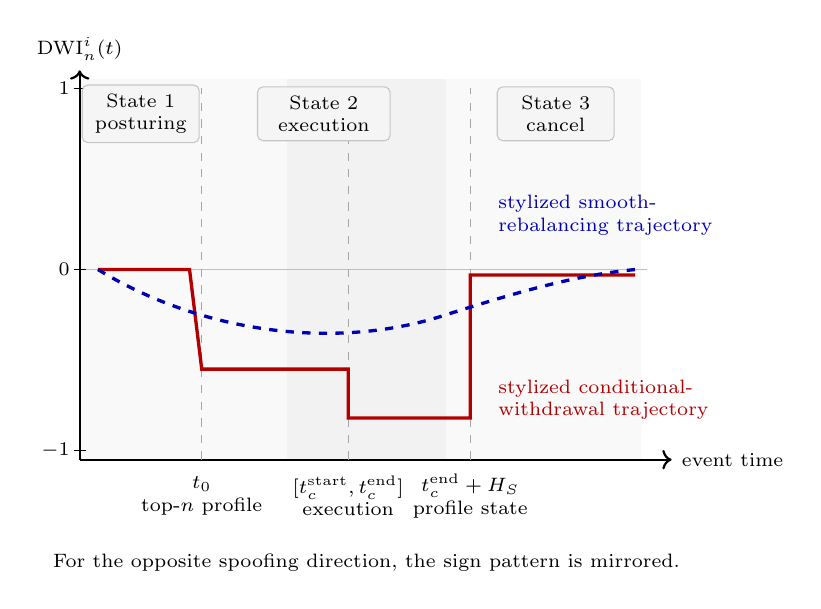
\begin{tikzpicture}[
        x=1.55cm,
        y=2.3cm,
        font=\scriptsize,
        axis/.style={->, thick},
        spoof/.style={very thick, red!70!black},
        maker/.style={very thick, dashed, blue!70!black},
        event/.style={gray!70, dashed},
        state/.style={fill=gray!8, draw=gray!45, rounded corners=2pt, align=center}
    ]
        \fill[gray!5] (0,-1.05) rectangle (1.7,1.05);
        \fill[gray!10] (1.7,-1.05) rectangle (3.0,1.05);
        \fill[gray!5] (3.0,-1.05) rectangle (4.6,1.05);

        \draw[axis] (0,-1.05) -- (0,1.1) node[above] {$\operatorname{DWI}_{n}^{i}(t)$};
        \draw[axis] (0,-1.05) -- (4.85,-1.05) node[right] {event time};
        \draw[gray!50] (-0.05,0) -- (4.65,0);

        \foreach \y/\lab in {-1/$-1$,0/$0$,1/$1$} {
            \draw (-0.05,\y) -- (0.05,\y) node[left=0.08cm] {\lab};
        }

        \draw[event] (1.0,-1.05) -- (1.0,1.0);
        \draw[event] (2.2,-1.05) -- (2.2,1.0);
        \draw[event] (3.2,-1.05) -- (3.2,1.0);

        \node[state, text width=1.25cm] at (0.5,0.86) {State 1\\posturing};
        \node[state, text width=1.45cm] at (2.0,0.86) {State 2\\execution};
        \node[state, text width=1.25cm] at (3.9,0.86) {State 3\\cancel};

        \node[align=center] at (1.0,-1.25) {$t_0$\\top-$n$ profile};
        \node[align=center] at (2.2,-1.25) {$[t_c^{\mathrm{start}},t_c^{\mathrm{end}}]$\\execution};
        \node[align=center] at (3.2,-1.25) {$t_c^{\mathrm{end}}+H_S$\\profile state};

        \draw[spoof] (0.15,0) -- (0.9,0)
            -- (1.0,-0.55) -- (2.2,-0.55)
            -- (2.2,-0.82) -- (3.2,-0.82)
            -- (3.2,-0.03) -- (4.55,-0.03);

        \draw[maker] (0.15,0) .. controls (1.0,-0.35) and (2.1,-0.45) .. (3.0,-0.25)
            .. controls (3.7,-0.10) and (4.1,-0.03) .. (4.55,0);

        \node[red!70!black, align=left, anchor=west] at (3.35,-0.72) {stylized conditional-\\withdrawal trajectory};
        \node[blue!70!black, align=left, anchor=west] at (3.35,0.30) {stylized smooth-\\rebalancing trajectory};
        \node[align=center] at (2.35,-1.62) {For the opposite spoofing direction, the sign pattern is mirrored.};
    \end{tikzpicture}
    \caption{Stylized multilevel distance-weighted imbalance around an execution. The conditional-withdrawal trajectory
    shows a large top-$n$ imbalance returning rapidly toward zero after the opposite-side execution. The smooth
    trajectory illustrates gradual rebalancing. Neither trajectory is an empirical classification rule.}
    \label{fig:topn_imbalance_dynamics}
\end{figure}
\FloatBarrier

\subsubsection{Conditional Withdrawal Reconstruction}
\label{subsec:multilevel_conditionality}

A static multilevel imbalance cannot establish manipulative intent. A market maker can also become temporarily imbalanced
while controlling inventory or responding to adverse selection. The additional observable feature is whether the profile
disappears conditionally after the participant's execution on the opposite side, as predicted by the stylized mechanism.

Let $c$ denote an execution for canonical actor $i$. Its ordered constituent execution messages share the trading partition,
actor key, order identifier, execution role, and side, and satisfy the operational inter-execution-message-gap rule. Passive executions
also share the resting price. Aggressive executions use reported traded price and quantity and may span
several price levels within the same order or sweep. The timestamps $t_c^{\mathrm{start}}$ and $t_c^{\mathrm{end}}$ denote
the first and last constituent execution messages. The quantity $Q_c$ is their total executed quantity, and $s_c\in\{b,a\}$ is the actor's
execution side. We denote the opposite candidate-posture side by $\bar{s}_c$. The pre- and post-execution observation times are
defined from the reconstructed state series in source order. Each state is recorded after applying its message. Therefore,
$t_c^{-}$ denotes the last actor-state row whose source index is strictly smaller than the first constituent execution message's index. Let
$t_c^{\mathrm{target}}=t_c^{\mathrm{end}}+H_S$, where $H_S=10$ seconds is the structural state horizon. The post-execution
state $t_c^{+}$ is the last reconstructed state at or before $t_c^{\mathrm{target}}$ whose source index is no smaller than
the final constituent execution message's index. SCI, each side-specific collapse measure $C^{i,s}_{c,n}$, and MSCI are undefined when either
required reconstructed state is unavailable.

We also impose a pre-execution episode window $\Theta>0$. An opposite-side order enters the candidate profile for execution
$c$ only when its first observed posting time $\tau_o$ satisfies
\begin{equation}
    0 \leq t_c^{\mathrm{start}}-\tau_o \leq \Theta .
    \label{eq:deceptive_age_window}
\end{equation}
The empirical analysis uses $\Theta=90$ seconds as an exploratory default. Let
$\mathcal{P}^{i,\bar{s}_c}_{c,n,\Theta}$ contain the orders that are active immediately before the first constituent execution message, belong
to actor $i$, lie on side $\bar{s}_c$ within the first $n$ book ranks, and satisfy
\cref{eq:deceptive_age_window}. The detector fixes this candidate set at the first constituent execution message. It records each order's
visible quantity, rank, kernel-weighted relative-depth contribution, and first-observed time. In particular, the raw
candidate quantity is
\begin{equation}
    Q^{i,\bar{s}_c}_{c,n}
    =
    \sum_{o\in\mathcal{P}^{i,\bar{s}_c}_{c,n,\Theta}} q_o(t_c^{-}).
    \label{eq:age_conditioned_candidate_quantity}
\end{equation}
The age restriction therefore governs candidate-order attribution, matched withdrawal, WMSCI, and the strict event gate.
It does not filter the state series used by SCI and MSCI.

The \textit{Spoofing Conditionality Index} instead measures the absolute change in the normalized shape of actor $i$'s
complete top-$n$ resting profile:
\begin{equation}
    \operatorname{SCI}^{i}_{c,n}
    =
    \left|
        \operatorname{DWI}^{i}_{n}(t_c^{-})
        -
        \operatorname{DWI}^{i}_{n}(t_c^{+})
    \right|.
    \label{eq:topn_sci}
\end{equation}
An absolute imbalance change does not identify which side lost liquidity. We therefore also measure the fraction of
weighted liquidity that disappears from each side after the execution using an exact piecewise definition:
\begin{equation}
    C^{i,s}_{c,n}
    =\begin{cases}
    \dfrac{
        \left[
            L^{i,s}_{n}(t_c^{-})-L^{i,s}_{n}(t_c^{+})
        \right]_{+}
    }{
        L^{i,s}_{n}(t_c^{-})
    },
    & L^{i,s}_{n}(t_c^{-})>0,\\
    0,
    & L^{i,s}_{n}(t_c^{-})=0.
    \end{cases}
    \qquad s\in\{b,a\}.
    \label{eq:side_collapse}
\end{equation}
where $[x]_{+}=\max\{x,0\}$. A large $C^{i,\bar{s}_c}_{c,n}$ indicates that the actor's top-$n$ liquidity decreased on the
side opposite to the execution. A two-sided quote refresh after a midprice change can instead generate material
collapse on both sides. The boundary values have a direct interpretation:
$C^{i,s}_{c,n}=1$ means that the entire weighted pre-execution profile on side $s$ disappeared, whereas
$C^{i,s}_{c,n}=0$ means that it did not decrease or was absent before execution.

To summarize these diagnostics while preserving evidence in both directions, define the event-level signed contrast
\begin{equation}
    \operatorname{MSCI}^{i}_{c,n}
    =\frac{1}{2}\operatorname{SCI}^{i}_{c,n}
     +C^{i,\bar{s}_c}_{c,n}
     -C^{i,s_c}_{c,n}.
    \label{eq:signed_msci}
\end{equation}
Because DWI lies in $[-1,1]$, $\operatorname{SCI}/2$ and each collapse term lie in $[0,1]$. Therefore, MSCI lies in
$[-1,2]$ without an additional clipping step. A positive MSCI means that normalized shape change and opposite-side collapse
outweigh same-side collapse. Zero is the neutral contrast, whereas a negative MSCI means that same-side collapse dominates.

The positive part in the definition of $C$ distinguishes liquidity disappearance from liquidity growth. It does not truncate
the subsequent cross-side contrast. The three inputs remain separately inspectable, so a two-sided quote refresh is
distinguishable from an asymmetric collapse. MSCI is a secondary event-level diagnostic that enters actor-level feature
summaries. It is neither a probability nor matched-withdrawal evidence. It does not enter the four-condition event gate or the
reported result tables. Operational outputs call it \texttt{MSCI\_resting\_profile} to emphasize that it uses all active
same-actor top-$n$ orders, not only the age-conditioned candidate set. Consequently, long-lived balanced liquidity can dilute
the measured shape change. MSCI should therefore be interpreted as context about the actor's complete resting profile rather
than as the collapse of the recent candidate layer.

\subsubsection{Canonical Matched Withdrawal}
\label{subsec:canonical_matched_withdrawal}

A cancellation can be eligible for several nearby executions. To measure withdrawal without counting that
cancellation more than once, let $\mathcal E(o)$ contain the eligible same-actor, opposite-side executions that precede
cancellation $o$ by at most $\Delta\tau_W$, where $\Delta\tau_W=2$ seconds in the reported specification. Eligibility is
evaluated only when the cancelled order belongs to the execution's fixed pre-execution candidate set; the timing and
source-sequence precedence conditions stated below must also hold. We assign $o$ deterministically to the canonical execution
\begin{equation}
    a(o)=\underset{c\in\mathcal E(o)}{\arg\min}\,
    \left(t_o-t_c^{\mathrm{end}},\;t_c^{\mathrm{start}},\;\operatorname{id}_c\right),
    \label{eq:canonical_cancel_assignment}
\end{equation}
where the tuple is ordered lexicographically and the stable execution identifier breaks any final tie. Eligibility also
requires source-sequence precedence: the cancellation follows the final constituent execution message in both event time and source
sequence. For eligible top-$n$ cancellations, define $\mathcal{C}_{c,n}^{i}=\{o:a(o)=c\}$. A physical cancellation is
identified by its trading partition, source index, and candidate order identifier. We preserve every eligible link for
audit, but each physical cancellation contributes to at most one execution's metrics.

An order can grow after the execution but before its cancellation. Such growth was not part of the pre-execution candidate
profile and must not increase the withdrawal attributed to that profile. For each assigned order
$o\in\mathcal{C}_{c,n}^{i}$, let $q^{\mathrm{pre}}_{c,o}$ denote its visible quantity immediately before the execution and let
$q^{\mathrm{cancel}}_o$ denote its visible quantity immediately before cancellation. We define the attributed quantity as
\begin{equation}
    \bar q_{c,o}
    =
    \min\!\left\{q^{\mathrm{pre}}_{c,o},q^{\mathrm{cancel}}_o\right\}.
    \label{eq:attributed_cancel_quantity}
\end{equation}
The raw cancellation-time quantity remains available for audit. The cap ensures that only liquidity already present in the
candidate layer contributes to matched withdrawal. The total assigned withdrawal and its ratio to execution quantity are
\begin{equation}
    U^{i}_{c,n}=\sum_{o\in\mathcal{C}_{c,n}^{i}}\bar q_{c,o},
    \qquad
    R^{i}_{c,n}=\frac{U^{i}_{c,n}}{Q_c},
    \label{eq:assigned_withdrawal}
\end{equation}
where $Q_c>0$ is the executed quantity by construction. Using the age-conditioned candidate quantity
$Q^{i,\bar{s}_c}_{c,n}$ from \cref{eq:age_conditioned_candidate_quantity}, we report the fraction of that profile removed as
\begin{equation}
    A^{i}_{c,n}
    =\begin{cases}
    \dfrac{U^{i}_{c,n}}{Q^{i,\bar{s}_c}_{c,n}},
    & Q^{i,\bar{s}_c}_{c,n}>0,\\
    \text{undefined},
    & Q^{i,\bar{s}_c}_{c,n}=0.
    \end{cases}
    \label{eq:assigned_withdrawal_share}
\end{equation}
The two ratios answer different questions. $R^{i}_{c,n}$ compares the attributed withdrawal with the executed quantity,
whereas $A^{i}_{c,n}$ compares it with the candidate profile that was available to withdraw. Under the reconstructed order
lifecycle and unique physical-cancellation assignment, the cap in \cref{eq:attributed_cancel_quantity} keeps
$A^{i}_{c,n}$ in $[0,1]$ whenever its denominator is positive.

For event prioritization, we also summarize the scale and speed of attributed withdrawal. Define the delay-weighted withdrawal quantity
\begin{equation}
    \widetilde U^{i}_{c,n}
    =
    \sum_{o\in\mathcal{C}_{c,n}^{i}}
    \bar q_{c,o}\exp\!\left(-\frac{t_o-t_c^{\mathrm{end}}}{\tau_w}\right),
    \qquad \tau_w=10\ \text{seconds}.
    \label{eq:delay_weighted_withdrawal}
\end{equation}
Within the $2$-second assignment window, the exponential factor decreases with cancellation delay. The decay scale
$\tau_w$ prioritizes temporal proximity; it is not an estimate of a causal response rate.
The event-level \textit{Withdrawal Multilevel Spoofing Conditionality Index} is
\begin{equation}
    \operatorname{WMSCI}^{i}_{c,n}
    =
    \begin{cases}
    \displaystyle
    \log\!\left(1+\frac{Q^{i,\bar{s}_c}_{c,n}}{Q_c}\right)
    \log\!\left(1+\frac{\widetilde U^{i}_{c,n}}{Q_c}\right)
    A^{i}_{c,n},
    & Q^{i,\bar{s}_c}_{c,n}>0\ \text{and}\ \widetilde U^{i}_{c,n}>0,\\[5pt]
    0,
    & Q^{i,\bar{s}_c}_{c,n}=0\ \text{or}\ \widetilde U^{i}_{c,n}=0.
    \end{cases}
    \label{eq:wmsci}
\end{equation}
The first logarithmic term measures the candidate posture relative to the execution. The second measures the
rapidly withdrawn quantity on the same scale, and $A^{i}_{c,n}$ measures the share of the candidate posture that is removed.
Under the piecewise definition, WMSCI is zero when either the candidate layer or delay-weighted attributed withdrawal makes
no positive contribution; this does not imply that the unrestricted resting profile was unchanged. WMSCI is non-negative
and has no fixed upper bound. We use it as the primary metric for ordering candidate events for
human review. It is neither a probability nor a calibrated measure of manipulative intent, and its magnitude should not be
interpreted as a proportional increase in suspiciousness. The full descriptive gate instead requires
$U^{i}_{c,n}>Q_c$ and the separate price-path conditions; it does not apply a WMSCI threshold. For each actor--partition combination,
we summarize repeated behavior through counts and withdrawal rates rather than aggregating WMSCI into an actor ranking.

\subsubsection{Price-Response Diagnostics}
\label{subsec:price_response_diagnostics}

Matched-withdrawal variables show whether an actor removes opposite-side liquidity after its own execution. They do not
show whether the price path is consistent with the hypothesized mechanism. Such a path first moves in the direction favorable
to the execution and then partly reverses after the candidate layer is removed. We measure these features with separate
price-response diagnostics. They are economic consistency checks, not causal
estimates of manipulation.

Let $b(t)$ and $a(t)$ denote the best bid and ask, with corresponding displayed quantities $q^b_1(t)$ and $q^a_1(t)$. When
both quotes and positive depth at the best quotes are available, the two market-price proxies are the midprice
$M_{\mathrm{mid}}(t)=[a(t)+b(t)]/2$ and the queue microprice
$M_{\mathrm{micro}}(t)=[a(t)q^b_1(t)+b(t)q^a_1(t)]/[q^b_1(t)+q^a_1(t)]$
\cite{Stoikov02122018}; otherwise the corresponding diagnostic is missing. Let $M(t)$ denote either proxy, and let $t_0$
be the earliest first-observed posting time among the eligible candidate orders for execution $c$. We encode the
execution direction as
\begin{equation}
    h_c=
    \begin{cases}
        +1, & \text{if the execution is a sell execution,}\\
        -1, & \text{if the execution is a buy execution.}
    \end{cases}
    \label{eq:price_response_direction}
\end{equation}
Under this convention, a positive signed change is favorable to the execution: a sell benefits from an upward move and a
buy from a downward move. We measure favorable movement from candidate-layer posting to execution as
\begin{equation}
    \operatorname{FPM}^{i}_{c}
    =
    h_c\left[M(t_c^{-})-M(t_0)\right],
    \label{eq:favorable_price_move}
\end{equation}
Reversion is anchored to each assigned cancellation rather than to the end of the execution. Let $t_o$ denote the
cancellation timestamp, $t_o^{-}$ the last reconstructed state strictly before its source index, and $H_R=2$ seconds the
reversion horizon. Let $\mathcal{C}_{c,n}^{i,\mathrm{obs}}$ contain the assigned cancellations for which the relevant
pre-cancellation and horizon values of $M$ are observed and $w_{c,o}>0$ is finite. For each execution, reversion after
cancellation is the mean weighted by attributed quantity and cancellation delay:
\begin{equation}
    \operatorname{REV}^{i}_{c}
    =
    \frac{
        \sum_{o\in\mathcal{C}_{c,n}^{i,\mathrm{obs}}}
        w_{c,o}h_c\left[M(t_o^{-})-M(t_o+H_R)\right]
    }{
        \sum_{o\in\mathcal{C}_{c,n}^{i,\mathrm{obs}}} w_{c,o}
    },
    \qquad
    w_{c,o}=\bar q_{c,o}\exp\!\left(-\frac{t_o-t_c^{\mathrm{end}}}{\tau_w}\right),
    \label{eq:price_reversion}
\end{equation}
with $\tau_w=10$ seconds in the reported run. Here $M(t_o+H_R)$ denotes the last reconstructed state at or before the
target time, provided that the message sequence covers that target. The statistic is undefined when no assigned cancellation
contributes a finite positive weight with both required price observations.
A positive $\operatorname{FPM}^{i}_{c}$ means that the price moved in the direction favorable to the execution
while the candidate layer was present. A positive $\operatorname{REV}^{i}_{c}$ means that the market-price proxy moved against the favorable pre-execution direction
after the assigned cancellation or cancellations. For execution price $P_c$, weighted by executed quantity, we also define
the local execution advantage relative to the pre-posture benchmark:
\begin{equation}
    \operatorname{ADV}^{i}_{c}
    =
    h_c\left[P_c-M(t_0)\right].
    \label{eq:execution_advantage}
\end{equation}
The execution advantage is positive when a sell executes above the benchmark or a buy executes below it.

We compute each diagnostic with both the midprice and the queue microprice in each event record. The reported summary
tables and the event gate use the midprice versions. We report price responses separately from withdrawal counts,
quantities, and rates instead of multiplying all components into one detector. Withdrawal variables describe the
reconstructed message sequence. The variables $\operatorname{FPM}$, $\operatorname{REV}$, and $\operatorname{ADV}$
describe the associated price path. This separation distinguishes repeated conditional withdrawals without a favorable
price response from episodes that also exhibit favorable pre-execution movement and post-cancellation reversion.

\subsubsection{Event Reconstruction}
\label{subsec:event_reconstruction}

We reconstruct events from individual order messages rather than aggregate snapshots. A resting order can change book rank
when the best quote moves even though its owner has neither modified nor cancelled it. Snapshot changes alone can therefore
confound repricing of the surrounding book with withdrawal by the participant. The reconstruction follows the economic
sequence from actor identification to execution, withdrawal, and price response:
\begin{enumerate}
    \item Resolve the canonical actor and classify each execution message as exclusively passive or aggressive. Construct execution $c$
    from compatible constituent execution messages while preserving the ordered mapping to raw messages.
    \item Reconstruct all active orders of actor $i$ immediately before $t_c^{\mathrm{start}}$, assign them to side and
    rank, and compute the unrestricted $L^{i,b}_{n}(t_c^{-})$, $L^{i,a}_{n}(t_c^{-})$, and
    $\operatorname{DWI}^{i}_{n}(t_c^{-})$.
    \item From opposite-side top-$n$ orders in the pre-execution state, retain the fixed candidate set
    $\mathcal{P}^{i,\bar{s}_c}_{c,n,\Theta}$ whose first-observed times satisfy the age restriction.
    \item Follow the complete actor state through the structural target $t_c^{\mathrm{end}}+H_S$ and select $t_c^{+}$
    according to the source-order and event-time rule above.
    \item Retain every eligible execution--cancellation link. Assign each physical cancellation canonically using
    \cref{eq:canonical_cancel_assignment}, exclude competing links from metric totals, and cap attributed quantity at the
    candidate order's pre-execution visible quantity using \cref{eq:attributed_cancel_quantity}.
    \item Compute SCI, \begin{review}collapse on each side\end{review}, and MSCI from \begin{review}the states of the unrestricted resting profile\end{review} at $t_c^{-}$ and
    $t_c^{+}$.
    \item Report assigned withdrawal quantity, \begin{review}ratio of withdrawal to execution\end{review}, \begin{review}fraction of the profile that was removed\end{review}, and WMSCI. Use WMSCI
    to order \begin{review}candidate events\end{review} for human review without applying it as \begin{review}a threshold for the strict gate\end{review}.
    \item Compute signed price diagnostics from \begin{review}the first posting in the candidate layer\end{review}, through the execution, to \begin{review}the window after cancellation\end{review}.
    \item Summarize repeated behavior with execution counts and \begin{review}diagnostics of recurrence for each actor\end{review}. Retain \begin{review}raw constituent execution messages\end{review} as provenance.
\end{enumerate}
This procedure is designed to distinguish ordinary book repricing from withdrawal of \begin{review}candidate liquidity attributed to the participant\end{review}. Canonical assignment ensures that one physical cancellation does not inflate the metrics of several neighboring
executions under the stated eligibility rule.

\begin{review}At the event level, the gate for a \textit{sequence compatible with spoofing}\end{review} passes only when four conditions hold simultaneously:
(i) \begin{review}cancellation of at least one eligible order on the opposite side\end{review} is canonically assigned within $2$ seconds of the execution;
(ii) the finite attributed withdrawal exceeds \begin{review}the positive quantity executed in the execution\end{review},
$U^{i}_{c,n}>Q_c$; (iii) the observed midprice $\operatorname{FPM}^{i}_{c}$ is strictly positive; and (iv) \begin{review}the observed midprice $\operatorname{REV}^{i}_{c}$ measured from cancellation\end{review} is strictly positive. \begin{review}A price diagnostic that is missing or right censored\end{review}
fails the conjunction. This transparent rule supports analyst triage; it is descriptive and is not a statistical test,
manipulation label, or proof of intent.

\begin{review}The reported specification uses a $10$-second window for structural reconstruction, a $2$-second window for both rapid attribution and reversion measured from cancellation, and a maximum age of $90$ seconds for candidate orders.\end{review} We estimate the empirical top-$10$ kernel separately for each
instrument. \begin{review}The components describing withdrawal and the price response\end{review} remain separate rather than being reduced to \begin{review}a single composite score\end{review}.

\section{Results}
\label{sec:results}

\subsection{Cross-Instrument Detection Summary}
\label{subsec:cross_instrument_results}

Rapid same-actor withdrawals occur in all three samples and after both passive and aggressive executions. The strict
sequence is necessarily rarer: beyond rapid canonical matching, it requires $U^{i}_{c,n}>Q_c$, positive favorable
pre-execution movement, and positive cancel-anchored reversion. \Cref{tab:empirical_spoofing_diagnostics} shows this
narrowing under a common top-$10$ resting-profile state and the same age-conditioned candidate-set reconstruction. Each
instrument uses the full-sample empirical kernel from \cref{tab:empirical_depth_kernel_calibration} at $H=10$ seconds.

A matched execution is a passive or aggressive execution followed within $2$ seconds by a canonically assigned cancellation
of a same-actor, opposite-side candidate order. The separate $10$-second interval is the structural reconstruction horizon.
Attributed withdrawal cannot exceed the candidate order's visible quantity before execution, while the raw
cancellation-time quantity remains available for audit. The table distinguishes executions from their raw constituent
execution messages, counts each assigned physical cancellation once, and identifies the coarser firm-fallback cases in
which the original client code is missing. Its strict column retains matched executions that also satisfy the withdrawal-size
and two price-response conditions. These are descriptive screening diagnostics, not manipulation labels or evidence of intent.

\InputIfFileExists{generated/spoofing_empirical_tables.tex}{}{%
    \fbox{\parbox{0.9\textwidth}{Run \texttt{scripts/generate\_spoofing\_paper\_tables.py} to generate the empirical tables.}}%
}
\FloatBarrier

The main empirical pattern is the gap between mechanical matching and the complete price-consistent sequence. The
reconstruction identifies \FerrariMatchedClusters{} matched executions for Ferrari, \NexiMatchedClusters{} for Nexi, and
\RisanamentoMatchedClusters{} for Risanamento. The strict gate retains \FerrariCompatibleSequences{},
\NexiCompatibleSequences{}, and \RisanamentoCompatibleSequences{}, respectively. Favorable pre-execution movement is
positive in \FerrariFPMShare{}, \NexiFPMShare{}, and \RisanamentoFPMShare{} of matched executions with an observed diagnostic;
positive reversion occurs in \FerrariREVShare{}, \NexiREVShare{}, and \RisanamentoREVShare{}. The withdrawal condition is
therefore not being used as a substitute for the full hypothesized price path. These marginal shares do not decompose
strict-set attrition across the jointly required conditions.

The table reports direct reconstruction counts and conditional descriptive shares. It contains no counterfactual comparison
or inferential test, and therefore provides neither $p$-values nor confidence intervals nor evidence that withdrawal is more
likely after the focal actor's own execution than under an otherwise comparable no-execution condition.

\paragraph{Event-accounting denominators.}
\Cref{tab:empirical_spoofing_diagnostics} reports raw-execution provenance, execution-anchor composition, firm-fallback
counts, and uniquely assigned physical cancellations for each instrument. Raw execution messages provide provenance,
whereas executions are the analytical unit for all conditional shares.

\subsection{Risanamento}
\label{subsec:risanamento_results}

Risanamento has the smallest matched set, and only \RisanamentoCompatibleSequences{} executions satisfy the strict
four-condition gate. Favorable pre-execution movement is nevertheless positive in \RisanamentoFPMShare{} of matched executions
with an observed diagnostic. Among matched executions with an observed reversion diagnostic, \RisanamentoREVShare{} have
\begin{review}positive reversion measured from cancellation\end{review}. The strict gate additionally requires \begin{review}positive favorable movement before execution\end{review} and
attributed withdrawal exceeding execution quantity, so these marginal shares do not identify which requirement excludes any
particular matched execution.

For each of the \RisanamentoMatchedClusters{} matched executions, the review record preserves \begin{review}a dossier organized around the execution and a reconstructed event window covering the top $10$ ranks\end{review}. These records organize observed facts, counter-evidence, and legitimate alternatives.
They are triage aids, not empirical labels or proof of manipulation.

\subsection{Nexi}
\label{subsec:nexi_results}

Nexi exhibits matched withdrawals after both execution routes, but \begin{review}the full path consistent with the price conditions\end{review} remains a subset.
Reconstruction identifies \NexiMatchedClusters{} matched executions, of which \NexiCompatibleSequences{} pass the strict gate.
Positive \begin{review}favorable movement before execution\end{review} occurs in \NexiFPMShare{} of matched executions with an observed diagnostic, while
\begin{review}positive reversion measured from cancellation\end{review} occurs in \NexiREVShare{}.

Differences from the other instruments are not causal contrasts because the samples cover different periods and actor
compositions.

\subsection{Ferrari}
\label{subsec:ferrari_results}

Ferrari has the largest matched set, with contributions from both passive and aggressive execution anchors.
Reconstruction identifies \FerrariMatchedClusters{} matched executions, and \FerrariCompatibleSequences{} pass the strict
gate. Among \begin{review}observed diagnostics for matched executions\end{review}, the shares with \begin{review}positive favorable movement before execution\end{review} and positive
reversion are \FerrariFPMShare{} and \FerrariREVShare{}.

These are descriptive screening outcomes, not manipulation labels or prevalence estimates.

\subsection{Actor-Level Attribution and Interpretation}
\label{subsec:actor_level_results}

Recurrence is informative only when actor identity and execution role remain explicit. \begin{review}The largest groups defined by actor and execution anchor differ in identity resolution, number of matched executions, withdrawal scale, and composition of the price path.\end{review} \Cref{tab:top_actor_results}
therefore reports the three largest groups in each instrument \begin{review}by number of matched executions\end{review} rather than collapsing them into one
actor score. An actor is either an original client code or, only when that code is missing, a firm identifier. W/E maximum is
the largest matched \begin{review}ratio of withdrawal to execution\end{review} within the group; FPM$+$ and REV$+$ are the shares of matched executions with
positive midprice favorable movement and reversion.

\InputIfFileExists{generated/spoofing_actor_table.tex}{}{%
    \fbox{\parbox{0.9\textwidth}{Run \texttt{scripts/generate\_spoofing\_paper\_tables.py} to generate the actor table.}}%
}
\FloatBarrier

The dispersion of FPM$+$ and REV$+$ across these groups shows why recurrence and price response must remain separate. A group
can contain many matched withdrawals without exhibiting the same reversion pattern as another group. Because firm fallback
can combine several clients, \begin{review}a count at firm level has coarser attribution than a count at client level and should not be interpreted as the history of a single account\end{review}.

\begin{review}The primary empirical object is the association, attributed to each actor, between execution and rapid withdrawal on the opposite side. Attribution is at client level when an original client code is observed and at the coarser firm level otherwise.\end{review} We report
its magnitude and repetition descriptively. \begin{review}WMSCI orders candidate events for review; MSCI remains a diagnostic that provides context from the complete resting profile; neither metric is a threshold for the strict gate or a score that ranks actors.\end{review} An analyst must also
consider the withdrawn order's execution risk and distance from the touch, bilateral activity, inventory context, price
response, and execution advantage. Together, these diagnostics support assessment of consistency with the stylized mechanism
while retaining legitimate liquidity provision as an alternative explanation. Neither WMSCI nor a dashboard review category
is treated as ground truth.

\subsection{Coverage of Externally Supplied Surveillance Alerts}
\label{subsec:external_alert_results}

\begin{review}At the scope of the subject reported externally\end{review}, the comparison recovers an execution in every distinct timed interval,
but the complete behavioral sequence appears in only four intervals. The $36$ timed source records become $34$ distinct intervals
after overlapping or endpoint-sharing records for the same instrument and external subject are merged. All $34$ intervals
contain raw subject activity and at least one recovered execution, while $30$ contain an attributed withdrawal.
\Cref{tab:external_alert_overlap} reports the corresponding hierarchy by instrument.

% Counts verified against external-alert audit SHA-256
% 30af0327718c4c793347acd462fb2674a8218c47537d5a96ff93ed7626cf7051.
\begin{table}[htbp]
\centering
\caption{Coverage of externally supplied timed alert records. Overlapping or endpoint-sharing records are merged only within
the same instrument and external subject. Execution counts intervals containing at least one execution with a constituent execution message inside
the closed union interval. Withdrawal and strict-scope columns count intervals containing at least one execution with \begin{review}the corresponding diagnostic at the event level\end{review}. Strict subject scope requires at least one execution in the interval to satisfy all four
gate conditions. The final column reports strict overlaps among intervals whose external
identity maps to one canonical actor at the same granularity; entries report strict intervals divided by \begin{review}intervals with aligned identity granularity\end{review}. The date-only Risanamento record is excluded from all timed denominators.}
\label{tab:external_alert_overlap}
\scriptsize
\setlength{\tabcolsep}{4.2pt}
\begin{tabular}{@{}lrrrrrr@{}}
\toprule
Instrument & \shortstack{Timed source\\records} & Union intervals & Execution & Withdrawal & Strict scope & \shortstack{Strict / aligned\\intervals} \\
\midrule
Ferrari & 35 & 33 & 33 & 30 & 4 & 0/3 \\
Nexi & 1 & 1 & 1 & 0 & 0 & 0/1 \\
\midrule
Total & 36 & 34 & 34 & 30 & 4 & 0/4 \\
\bottomrule
\end{tabular}
\end{table}

\begin{review}All four strict overlaps at subject scope occur within the $30$ Ferrari intervals for which identity granularity is not aligned and the main externally reported firm maps to two canonical actor keys.\end{review} \begin{review}Correspondence with an exact actor\end{review} is therefore not identifiable in those intervals. By contrast,
the comparison contains four \begin{review}intervals with aligned identity granularity\end{review}---three for Ferrari and one for Nexi---and none contains a strict
sequence. The Nexi interval nevertheless contains one aggressive execution formed from four constituent execution messages, but it has
no attributed withdrawal under the stated timing rule.

The Risanamento source identifies only one trading date. On that date, the reported subject has $59$ reconstructed
executions, including one execution with an attributed withdrawal and no strict sequence. \begin{review}These counts over the full day\end{review} establish that the
subject is observable, but they cannot identify correspondence with the specific external event.

These results measure recovery relative to externally reported activity. \begin{review}Strict recall for an exact actor is identifiable only for the four unioned timed intervals with aligned identity granularity, none of which contains a strict sequence.\end{review} The four strict overlaps among
the remaining intervals are \begin{review}overlaps at subject scope, not recall for an exact actor\end{review}. Because \begin{review}the source contains only positive cases and was not independently adjudicated again for manipulative intent\end{review}, these quantities do not estimate recall or precision against true
manipulation. No negative windows are available to estimate false positives. Moreover, the external alert rule and the strict
four-condition gate need not define the same event population. The sparse strict overlap records limited agreement under two
operational definitions. It cannot, by itself, identify false negatives, false positives, or the source of disagreement.
\FloatBarrier

\section{Discussion and Conclusion}
\label{sec:discussion_conclusion}

The main empirical finding is that rapid same-actor withdrawal is broader than the complete spoofing-compatible sequence.
Matched episodes occur after both passive and aggressive executions in all three samples, but only a subset also exhibits the
required withdrawal size, favorable pre-execution movement, and post-cancellation reversion. This distinction prevents a
high cancellation rate or a large withdrawal from standing in for the full mechanism.

The external-alert audit reinforces the same separation. The reconstruction covers execution in all $34$ distinct timed
intervals and attributed withdrawal in $30$, whereas only four intervals contain a strict sequence at subject scope. None of
the four identity-aligned intervals contains a strict sequence, and the four strict subject-scope overlaps cannot be resolved
to one canonical actor. The strict gate is therefore not a surrogate for the external surveillance rule.

The construction keeps the relevant evidence types separate. $U^{i}_{c,n}$, $R^{i}_{c,n}$, and $A^{i}_{c,n}$ describe
how much of the pre-execution candidate layer can be attributed to withdrawal and how its scale compares with the execution.
$\operatorname{FPM}^{i}_{c}$ and $\operatorname{REV}^{i}_{c}$ describe the associated price path. Their conjunction forms
the strict gate, but remains a descriptive compatibility rule: it neither estimates spoofing prevalence nor establishes that
any retained sequence was manipulative. WMSCI separately prioritizes event-level review by combining candidate-layer scale,
rapid attributed withdrawal, and the removed-profile fraction. MSCI instead describes the complete resting profile, which can
be diluted by long-lived balanced liquidity. Neither is a strict-gate threshold or a pass--fail condition.

The strongest limitation is the absence of a counterfactual comparison and an independently adjudicated label set. The
analysis does not test whether withdrawal is more likely after the focal actor's execution than after an otherwise comparable
non-event, and repeated observations from the same actors or trading periods need not be independent. The external alerts add
positive reference periods but no negative controls. They support recovery relative to the source alerts and exact-actor
strict-recall accounting under the identity-alignment rule, but cannot identify recall or precision against independently
adjudicated manipulation labels or calibrate detector thresholds. The depth kernels are calibrated on the same full samples
to which they are applied, so their displayed-price associations are descriptive rather than out-of-sample evidence.
Right\nobreakdash-censored reversion outcomes fail the event gate, and the reported results do not test sensitivity to the
$100$-millisecond execution-grouping threshold, the $90$-second candidate age, or the reported $2$- and $10$-second windows.

Identity and sampling impose further limits. Firm fallback can pool several clients, so firm-level recurrence is not directly
comparable with recurrence under a client code. Aggressive execution is an execution-role observation, not evidence about the
intent of the surrounding resting orders; ordinary liquidity taking remains an alternative explanation. External firm-level
alerts can also span several internal actor keys, which prevents exact-actor evaluation in those intervals. The three
instrument samples cover different periods and actor compositions, which rules out causal cross-instrument comparisons.

The contribution is therefore an auditable surveillance workflow rather than an enforcement classifier. It preserves raw
message provenance, separates withdrawal from price-response evidence, and exposes the gate conditions used for triage.
Prospective use would require a pre-specified counterfactual design and thresholds, kernel calibration on training periods
only, chronological out-of-sample validation, and evaluation against independently reviewed cases with explicit
false-positive and false-negative costs.

% We propose two agent-specific metrics based on the
% microprice and the volume-distance correlation. 
% \paragraph{Agent-Specific Microprice ($m_i$)} The traditional microprice is widely 
% recognized in high-frequency trading as a robust estimator of the expected future midprice \cite{Stoikov02122018}, uniquely synthesizing both
% the price and volume dimensions of the limit order book. By isolating this calculation to a single participant's resting 
% orders, we can formulate an an agent-specific microprice ($m_i$) to quantify its personal vision of the future price::

% \begin{equation}
%     m_i = \frac{a_iV^b_i + b_i V^a_i}{V^b_i + V^a_i} = \frac{a_i + b_i}{2} + \frac{a_i-b_i}{2} \frac{V_i^b-V_i^a}{V_i^b+V_i^a} = \text{midprice} + \frac{\text{spread}}{2} \times \text{imbalance}
% \end{equation}
% Where $a_i$ and $b_i$ represent the agent's ask and bid prices, and $V^a_i$ and $V^b_i$ represent their respective 
% volumes. Legitimate market makers, constrained by inventory risk, typically maintain symmetric quotes ($V^b_i \approx V^a_i$) 
% to capture the spread, resulting in an $m_i$ that closely tracks the fundamental midprice. Conversely, a spoofer
% deliberately engineers an extreme unbalanced environment to manipulate the heuristics of victim algorithms. 
% Consequently, a spoofer's $m_i$ will drastically diverge from the true midprice.

% \paragraph{Correlation Between Posting Distance ($\delta$) and Volume} The second metric mathematically formalizes the 
% spoofer's optimization dilemma by measuring the correlation between an agent's order volume and their posting distance 
% ($\delta$) from the best bid or ask. Empirical models confirm that posting distance is a critical determinant of price 
% impact, and its omission renders LOB detection models mathematically inadequate.Because market makers seek execution to 
% earn the bid-ask spread, their inventory management necessitates posting their largest order volumes at or adjacent to 
% the top of the book ($\delta \approx 0$). Spoofers, conversely, optimize a strictly directional expected cost function: 
% they must maximize the psychological and algorithmic impact of their non-bona fide volume while minimizing the risk of 
% inadvertent execution. This is achieved by placing a small, bona fide order at a minimal distance ($\delta \approx 0$) 
% to guarantee execution, and a massive, non-bona fide order at a significantly larger distance deeper within the opposite 
% side of the LOB ($\delta \gg 0$) to act as a structural buffer against aggressive market orders. Thus, observing a strong 
% correlation between massive volume and a large $\delta$ on one side of the book—paired with small volume and a minimal 
% $\delta$ on the execution side—serves as and additional microstructural signature of a manipulative strategy.


\bibliographystyle{abbrv}
\bibliography{references}

\end{document}
